\documentclass{article}

\usepackage{neurips_2026}

\usepackage[utf8]{inputenc} % allow utf-8 input
\usepackage[T1]{fontenc}    % use 8-bit T1 fonts
\usepackage{hyperref}       % hyperlinks
\usepackage{url}            % simple URL typesetting
\usepackage{booktabs}       % professional-quality tables
\usepackage{amsfonts}       % blackboard math symbols
\usepackage{nicefrac}       % compact symbols for 1/2, etc.
\usepackage{microtype}      % microtypography
\usepackage{xcolor}         % colors

\usepackage{multirow}
\usepackage{amssymb}
\usepackage{graphicx}
\usepackage{natbib}
\usepackage{doi}
\usepackage{amsmath}
\usepackage{physics}
\usepackage{wrapfig}
\usepackage{bm}
\usepackage{algorithm,algpseudocode}
\usepackage{forest}
\usepackage{tcolorbox}
\usepackage{tikz-cd}
\usetikzlibrary{calc}
\usepackage{enumitem}

\usepackage{amsthm}

\newtheorem{theorem}{Theorem}
\newtheorem{lemma}{Lemma}
\newtheorem{proposition}{Proposition}
\newtheorem{corollary}{Corollary}

\theoremstyle{definition}
\newtheorem{definition}{Definition}
\newtheorem{assumption}{Assumption}

\theoremstyle{remark}
\newtheorem{remark}{Remark}
\newtheorem{example}{Example}

% Blackboard bold sets
\newcommand{\R}{\mathbb{R}}
\newcommand{\N}{\mathbb{N}}
\newcommand{\Z}{\mathbb{Z}}
\newcommand{\Q}{\mathbb{Q}}
\newcommand{\C}{\mathbb{C}}

% Labels
\newcommand{\alg}{\mathrm{alg}}
\newcommand{\meta}{\mathrm{meta}}
\newcommand{\fix}{\mathrm{fix}}

% Probability
\newcommand{\Prb}{\mathbb{P}}
\newcommand{\E}{\mathbb{E}}
\DeclareMathOperator{\Var}{Var}
\DeclareMathOperator{\Cov}{Cov}

% Operators
\DeclareMathOperator{\diag}{diag}
\DeclareMathOperator{\supp}{supp}

\newcommand{\argmax}{\operatorname*{arg\,max}}
\newcommand{\argmin}{\operatorname*{arg\,min}}
\newcommand{\ind}{\mathbf{1}}

% Inner product
\newcommand{\inner}[2]{\left\langle #1, #2 \right\rangle}

% Calligraphic sets
\newcommand{\cA}{\mathcal{A}}
\newcommand{\cS}{\mathcal{S}}
\newcommand{\cT}{\mathcal{T}}
\newcommand{\cF}{\mathcal{F}}
\newcommand{\cE}{\mathcal{E}}

% RL notation
\newcommand{\SSS}{\mathcal{S}}
\newcommand{\AAA}{\mathcal{A}}
\newcommand{\PP}{\mathcal{P}}
\newcommand{\RRR}{\mathcal{R}}
\newcommand{\gammaRL}{\gamma}

% Confidence bounds
\newcommand{\olQ}{\overline{Q}}
\newcommand{\ulQ}{\underline{Q}}
\newcommand{\olV}{\overline{V}}
\newcommand{\ulV}{\underline{V}}

% Misc
\newcommand{\eps}{\varepsilon}
\newcommand{\dt}{\mathrm{d}t}
\newcommand{\given}{\,\bigl\vert\,}

% Fractions
\newcommand{\half}{\tfrac12}
\newcommand{\thalf}{\tfrac32}

% Notes
\newcommand{\note}[1]{\paragraph{Note.} #1}

\theoremstyle{remark}
\newtheorem{conjecture}[theorem]{Conjecture}


\newcommand{\todo}[1]{\textcolor{red!70!black}{[\textbf{TODO:} #1]}}
\newcommand{\Cold}{\mathsf{C}}
\newcommand{\Exp}{\mathsf{E}}
\newcommand{\Hyb}{\mathsf{H}}
\newcommand{\wid}{w}

\title{Information Value Is Not Policy Value:\\ When LLM Warm-Starts Help Linear Contextual Bandits}


\author{%
  David S.~Hippocampus\thanks{Use footnote for providing further information
    about author (webpage, alternative address)---\emph{not} for acknowledging
    funding agencies.} \\
  Department of Computer Science\\
  Cranberry-Lemon University\\
  Pittsburgh, PA 15213 \\
  \texttt{hippo@cs.cranberry-lemon.edu} \\
}


\begin{document}
\maketitle
\begin{abstract}
A recent line of work reports ``reward multiplication'': routing the early
rounds of a linear contextual bandit to a frozen LLM policy and then handing
control to LinUCB can beat both the LLM and cold-started LinUCB, sometimes by a
large factor. We give an exact accounting of when this can happen. The regret
difference between cold LinUCB and the handoff hybrid splits into the expert's
direct reward advantage during the routed rounds plus the value of the data
those rounds leave in LinUCB's design matrix; the difference between the expert
and the hybrid is the adaptive learner's advantage on the tail. Multiplication
requires both differences to be large at once, and the second term is governed
by a single round-level quantity: the regret LinUCB can still incur on a
competitor whose confidence width has not yet fallen below its suboptimality
gap. We show that the canonical separating instance in the literature is a pure
example of the data-value term---a policy with linear regret generates, offline,
a design matrix that drives LinUCB's regret from linear to constant---and that
on the same instance no online handoff realizes any of that value, because
useful covariance there can only be bought at a constant rate of regret. We
then construct an instance on which an online handoff provably multiplies,
and show that the multiplier over cold LinUCB equals, up to constants, the
ratio of two prices: the regret cold exploration pays per unit of coverage
of the directions that matter, divided by the regret the expert pays for the
same coverage. A catalog of ten instances, each removing one ingredient,
shows that recurrence of directions, cheapness of the expert's informative
actions, correct targeting, and the expert's suboptimality on the tail are
each necessary. This separates the information value of an expert from its
policy value, explains
why two LLMs of equal accuracy can yield very different gains, and yields
pre-runtime estimates of the transferable width reduction and the regret paid
to acquire it. On two datasets and twelve dataset/model configurations, the
one configuration with a large estimated net value is the one that multiplies
($2.34\times$); the others do not.
\end{abstract}


\section{Introduction}
\label{sec:intro}

Sequential decision making studies how an agent adapts to an unknown
environment through repeated interaction \cite{zhu2022largeaction,zhu2022contextual},
with applications in recommendation \cite{li2010contextual,agarwal2016making},
healthcare \cite{tewari2017ads,svensson2023sequential}, and dialogue
\cite{li2016deep}. Large pretrained language models supply prior knowledge that
can guide early decisions
\cite{brown2020language,ouyang2022training,achiam2023gpt,
alamdari2024jumpstarting,abbasiyadkori2024believe}.

A striking observation is that combining a frozen LLM with an adaptive linear
bandit can strictly dominate either component, sometimes by orders of magnitude
\cite{chen2024llmdecision,huangcontextual}. Yet bandit warm-starting
\cite{bastani2021mostly,zhang2019warm} and confidence-gated model selection
\cite{auer2002nonstochastic,agarwal2017corralling,pacchiano2020model} are older
objects, and that literature does not report comparable multipliers. The
tension dissolves once one separates two things that are easy to conflate:
the \emph{policy value} of an expert (how much reward its actions earn) and
the \emph{information value} of an expert (how much its actions teach an
adaptive learner that keeps their covariance). The two can be wildly
different. A separating instance we construct to model the phenomenon
% NOTE: the construction is ours (it does not appear in chen2024llmdecision,
% which is empirical); crediting it away both misattributes and undersells.
documented by \cite{chen2024llmdecision}, stated as
Proposition~\ref{prop:three-way}, is the cleanest illustration:
a constant policy that is wrong on every round, and whose regret is therefore
linear, produces a design matrix under which LinUCB's regret collapses from
linear to constant. The expert there has no policy value at all; its data has
enormous information value.

This paper makes that separation exact and uses it to say when a handoff from
a frozen expert to LinUCB can multiply reward. Writing $\Cold$ for cold LinUCB,
$\Exp$ for the frozen expert, and $\Hyb_\tau$ for the hybrid that follows
$\Exp$ for $\tau$ rounds while feeding every observation to LinUCB and then
hands over, we have the identities
\[
R_T(\Cold)-R_T(\Hyb_\tau)=A_\tau+V_\tau,
\qquad
R_T(\Exp)-R_T(\Hyb_\tau)=B_\tau,
\]
where $A_\tau$ is the expert's reward advantage over cold LinUCB on the routed
rounds, $V_\tau$ is the regret LinUCB saves after the handoff because of the
data the expert left behind, and $B_\tau$ is the adaptive learner's advantage
over the frozen expert on the tail (Theorem~\ref{prop:decomp}). Reward
multiplication over both base policies means $A_\tau+V_\tau$ and $B_\tau$ are
simultaneously large. The first is where the trade-off lives: the expert's
actions must be cheap (small regret while routed) and informative (large
$V_\tau$), and on many instances those two requirements pull in opposite
directions.

What governs $V_\tau$ is a round-level quantity that is standard in the
analysis of optimistic algorithms but rarely isolated. On the confidence event,
the instantaneous regret of LinUCB at round $t$ with design matrix $V$ is at
most
\[
\Phi_t(V)\;:=\;\max_{a\in\mathcal A_t}\min\bigl\{\Delta_{t,a},\;2\beta_t\|x_{t,a}\|_{V^{-1}}\bigr\},
\]
the largest gap among competitors whose confidence width still exceeds their
gap (Lemma~\ref{lem:width-limited}). Everything that the prior literature
attributes to ``dimension,'' ``coherence,'' or ``gap structure'' enters through
$\Phi_t$: the gap through the first argument of the minimum; the dimension
through how many distinct directions can keep a width large; coherence
through how much one observation shrinks the width of another direction, which
is an exact Sherman--Morrison identity (Lemma~\ref{lem:transfer}); and a warm
start through the Loewner ordering $(\lambda I+M)^{-1}\preceq(\lambda I)^{-1}$
(Lemma~\ref{lem:loewner}). We therefore do not posit separate structural axes.
We derive them.

Two consequences follow. First, the determinant-ratio (elliptical potential)
bound that underlies every $\widetilde O(\sqrt{rT})$-type guarantee cannot by
itself certify a multiplicative gain: with $\tau=o(T)$ the ratio of the warm
and cold determinant bounds tends to one, so any order-of-magnitude effect must
come from competitors whose widths the warm start pushes \emph{below their
gaps}, exactly as in Proposition~\ref{prop:three-way}
(Theorem~\ref{thm:handoff} and the discussion after it). Second, the offline
separation of Proposition~\ref{prop:three-way} has no online counterpart on
the same instance: for \emph{every} expert policy and every $\tau$, the
handoff hybrid has $V_\tau=0$, because each round introduces a fresh direction
that no earlier observation can cover (Proposition~\ref{prop:one-pass}). Online
multiplication needs an expert whose cheap actions land on the directions that
cold exploration would otherwise waste regret resolving.

We then show that such an expert exists and that its multiplier is a ratio
of prices. Call the price of a direction the least regret any policy must pay
per unit of coverage of it (Equation~\eqref{eq:price}). On an instance in which
the directions that trap cold LinUCB recur, and in which a cheap ``probe''
action covering them is available early on, a frozen expert that plays the
probes and then hands off has regret smaller than cold LinUCB's by a factor
of order $c^2/(\eps L^2)$, where $1/L^2$ is the price cold exploration pays and
$\eps/c^2$ the price the probe pays, and smaller than the expert's own by a
factor that grows with the horizon (Theorem~\ref{thm:price}). The confidence
radius cancels. The same instance, with the probe made dear, gives a
multiplier of at most two. A catalog of ten instances
(Section~\ref{sec:catalog}, Table~\ref{tab:catalog}), all built from the
canonical one by changing a single ingredient, isolates what each clause of
this mechanism contributes, and each experimental configuration of
Section~\ref{sec:experiments} has a row in it.

\paragraph{Contributions.}
\begin{itemize}[itemsep=1pt, topsep=1pt, leftmargin=*]
\item \textbf{An exact decomposition of reward multiplication}
(Theorem~\ref{prop:decomp}) into the expert's direct advantage $A_\tau$,
the value of the transferred data $V_\tau$, and the adaptive tail advantage
$B_\tau$, and a round-level bound on what governs $V_\tau$
(Lemma~\ref{lem:width-limited}).
\item \textbf{A clean separation of information value from policy value.}
Proposition~\ref{prop:three-way} (offline transfer) is paired with
Proposition~\ref{prop:one-pass} (no online transfer on the same instance),
and with exact identities showing how a warm start and how ordinary
exploration reduce confidence widths (Lemmas~\ref{lem:loewner}
and~\ref{lem:transfer}).
\item \textbf{An online instance with a provable multiplier, and the price
ratio as its value} (Theorem~\ref{thm:price}), together with a catalog of
ten instances with complete proofs (Section~\ref{sec:catalog},
Appendix~\ref{app:catalog}) that shows which ingredient each negative case is
missing and places each experimental configuration.
\item \textbf{A handoff regret bound stated in exact determinant form}
(Theorem~\ref{thm:handoff}), with the expert's routed-round regret charged
exactly rather than through an assumed accuracy level, and an honest reading
of what it does and does not certify.
\item \textbf{Pre-runtime estimates of transferable width reduction and
acquisition regret}, computable from a labeled held-out sample plus the
expert's proposals on it (Section~\ref{sec:diagnostics}), with experiments on
two datasets and eight model/embedding pairings (Section~\ref{sec:experiments}).
\end{itemize}
A detailed related-work discussion is in Appendix~\ref{sec:related}.


\section{Preliminaries}
\label{sec:preliminaries}

We work in a standard linear contextual bandit
\cite{abbasi2011improved,chu2011contextual,lattimore2020bandit}. At each round
$t=1,\dots,T$, the learner observes a finite action set $\mathcal A_t$ where
each $a\in\mathcal A_t$ has a feature vector $x_{t,a}\in\mathbb R^d$ with
$\|x_{t,a}\|_2\le L$, selects $A_t\in\mathcal A_t$, and observes
$r_t=\langle\theta^\star,x_{t,A_t}\rangle+\eta_t$, where $\theta^\star$ is
unknown with $\|\theta^\star\|_2\le S$ and $\eta_t$ is conditionally mean-zero
and $\sigma$-sub-Gaussian. Write $\mu_t(a)=\langle\theta^\star,x_{t,a}\rangle$,
$a_t^\star\in\arg\max_a\mu_t(a)$, and $\Delta_{t,a}=\mu_t(a_t^\star)-\mu_t(a)$
for the suboptimality gap of $a$ at round $t$. For a policy $\pi$ and an
interval $I\subseteq[T]$ of rounds, $R_I(\pi)=\sum_{t\in I}\Delta_{t,\pi_t}$ is
its pseudo-regret on $I$, and $R_T(\pi)=R_{[T]}(\pi)$. The language aspect of
the applications we target enters only through the feature map: context and
action embeddings from pretrained models are combined into $x_{t,a}$, and the
frozen expert may be an LLM. Nothing in the theory uses language structure.

\paragraph{LinUCB and its warm start.}
LinUCB maintains $V_t=V_1+\sum_{s<t}x_{s,A_s}x_{s,A_s}^\top$,
$b_t=b_1+\sum_{s<t}r_sx_{s,A_s}$, $\widehat\theta_t=V_t^{-1}b_t$, and plays
$A_t\in\arg\max_a\langle\widehat\theta_t,x_{t,a}\rangle+\beta_t\|x_{t,a}\|_{V_t^{-1}}$,
where $\|x\|_{V^{-1}}=\sqrt{x^\top V^{-1}x}$ is the confidence width of $x$ and
$\beta_t$ is the confidence radius. \emph{Cold-started} LinUCB, written
$\Cold$, uses $V_1=\lambda I_d$, $b_1=0$. A \emph{warm start} $(M,c)$ uses
$V_1=\lambda I_d+M$ and $b_1=c$ with $M=\sum_sx_sx_s^\top\succeq0$ and
$c=\sum_sr_sx_s$ the Gram matrix and response sum of some logged data. We say
the warm start is \emph{offline} if that data is not counted in the evaluated
horizon and \emph{online} if it is.

\paragraph{Frozen expert and handoff hybrid.}
A frozen expert $\Exp$ proposes $a_t^{\Exp}\in\mathcal A_t$ at each round by a
rule that is never updated (for an LLM, the action whose embedding is closest
to the LLM's output; see Section~\ref{sec:exp-setup}). For $\tau\in\{0,\dots,T\}$
the \emph{handoff hybrid} $\Hyb_\tau$ plays $a_t^{\Exp}$ for $t\le\tau$, updates
$(V_t,b_t)$ with every played action and observed reward including those
rounds, and plays LinUCB for $t>\tau$. Thus $\Hyb_0=\Cold$ and $\Hyb_T=\Exp$,
and the LinUCB phase of $\Hyb_\tau$ is LinUCB with the online warm start
$(M_\tau,c_\tau)=\bigl(\sum_{t\le\tau}x_{t,A_t}x_{t,A_t}^\top,\sum_{t\le\tau}r_tx_{t,A_t}\bigr)$.
The deterministic router used in our experiments
(Appendix~\ref{app:meta-algorithm}) chooses $\tau$ adaptively and may
interleave the two; the theory below is for a fixed $\tau$, which is the
right object for understanding why a multiplier appears, and we comment on
adaptive $\tau$ after Theorem~\ref{thm:handoff}.


\section{Main Results}
\label{sec:main-results}

\subsection{The Main Theorem}
\label{sec:catalog}

Everything in this paper is organized by one identity.

\paragraph{Setup for the decomposition.}
Recall the three policies: $\Cold$ is LinUCB initialized from $\lambda I_d$
(no prior data); $\Exp$ is a frozen expert that proposes actions by a fixed
rule (e.g.\ an LLM) and is never updated; and $\Hyb_\tau$ is the handoff
hybrid that follows $\Exp$ for the first $\tau$ rounds, feeds every
observation into LinUCB's state $(V_t,b_t)$, and then hands control to LinUCB
for rounds $\tau{+}1,\dots,T$. For any policy $\pi$ and interval $I$, we
write $R_I(\pi)=\sum_{t\in I}\Delta_{t,\pi_t}$ for its pseudo-regret on $I$,
and $R_T(\pi)=R_{[T]}(\pi)$.

\begin{theorem}[Decomposition of the hybrid's advantage]
\label{prop:decomp}
For any instance, any expert $\Exp$, any $\tau$, and any realization of the
noise,
\begin{align*}
R_T(\Cold)-R_T(\Hyb_\tau)
&=\underbrace{R_{[1,\tau]}(\Cold)-R_{[1,\tau]}(\Exp)}_{A_\tau}
 +\underbrace{R_{[\tau+1,T]}(\Cold)-R_{[\tau+1,T]}(\Hyb_\tau)}_{V_\tau},\\
R_T(\Exp)-R_T(\Hyb_\tau)
&=\underbrace{R_{[\tau+1,T]}(\Exp)-R_{[\tau+1,T]}(\Hyb_\tau)}_{B_\tau}.
\end{align*}
\end{theorem}

$A_\tau$ is the expert's \emph{direct} advantage: positive if the expert earns
more than cold LinUCB would have on the routed rounds, negative if the expert's
actions cost more regret than cold exploration. $V_\tau$ is the
\emph{information} value of the routed rounds: it is nonzero only through the
warm start $(M_\tau,c_\tau)$ that they leave in LinUCB's state, since apart
from that state $\Hyb_\tau$ and $\Cold$ run the same algorithm on the same
future. $B_\tau$ is the adaptive learner's advantage on the tail and is large
only when the expert remains substantially suboptimal late while the
warm-started learner does not. We write $R_{[1,\tau]}(\Exp)=\sum_{t\le\tau}\Delta_{t,a_t^{\Exp}}$
for the \emph{acquisition regret} of the warm start: the price, counted in the
online horizon, of the data in $M_\tau$.

\begin{remark}
The identities of Theorem~\ref{prop:decomp} hold in expectation as well as
pathwise. In particular, $R_T(\Hyb_\tau)\le\min\{R_T(\Cold),R_T(\Exp)\}$ if
and only if $A_\tau+V_\tau\ge0$ and $B_\tau\ge0$, and
$\min\{R_T(\Cold),R_T(\Exp)\}/R_T(\Hyb_\tau)\to\infty$ along a sequence of
instances if and only if both $A_\tau+V_\tau$ and $B_\tau$ exhaust the
corresponding base regret up to lower-order terms. If instead the warm start
$(M,c)$ is built from data outside the horizon (an \emph{offline} warm start
$\Hyb^{\mathrm{off}}$, LinUCB started from $(\lambda I+M,c)$), the routed
rounds are not charged and the identities read
$R_T(\Cold)-R_T(\Hyb^{\mathrm{off}})=:V^{\mathrm{off}}$ and
$R_T(\Exp)-R_T(\Hyb^{\mathrm{off}})=:B^{\mathrm{off}}$, with no $A$ term.
\end{remark}

The theorem is bookkeeping and says nothing by itself. Its content is in
what the three terms can be. Reward multiplication over both base policies
means $A_\tau+V_\tau$ is almost all of $R_T(\Cold)$ and $B_\tau$ is almost all
of $R_T(\Exp)$, so every question about when a handoff multiplies is a
question about which of $A_\tau$, $V_\tau$, $B_\tau$ can be large at once. We
answer it with ten instances, each obtained from the canonical one
(Proposition~\ref{prop:three-way}) by changing a single ingredient
(Table~\ref{tab:catalog}); exactly one of them has all three terms large,
and its multiplier is a ratio of prices (Theorem~\ref{thm:price}). The
pattern across the rows is the following.


\begin{center}
\fbox{\parbox{0.95\linewidth}{\textbf{Thesis.}
A handoff multiplies regret savings over cold LinUCB if and only if the
expert's routed actions buy coverage of the directions cold LinUCB would
otherwise pay for, at a lower price than cold exploration pays, early enough
for those directions to recur; and it multiplies over the expert if and only
if, in addition, the expert is worse than the warm-started learner on the tail.
}}
\end{center}

The catalog has ten rows rather than the $2^3=8$ of a binary table because
several terms admit qualitatively distinct failure modes---for instance,
$V_\tau$ can vanish because the expert buys the same directions cold
exploration buys at the same price (row~4), because it buys the wrong
directions (row~7), or because it buys the right directions too dearly
(row~8)---and because the offline/online distinction (rows~1--2) and the two
ways of killing the tail term (rows~3 and~6) each warrant separate entries.

\begin{table}[t]
\centering
\scriptsize
\setlength{\tabcolsep}{2.5pt}
\begin{tabular}{@{}clccccl@{}}
\toprule
\# & Instance & $A_\tau$ & $V_\tau$ & $B_\tau$ & Ratio to $\Cold$ & Ingredient isolated\\
\midrule
1 & canonical, offline (Prop.~\ref{prop:three-way}) & not charged & $V^{\mathrm{off}}\asymp T$ & $B^{\mathrm{off}}\asymp T$ & $\asymp T$ & data is free\\
2 & canonical, online (Prop.~\ref{prop:one-pass}) & $\le\tau$ & $0$ & $\le0$ & none & directions never recur\\
3 & canonical, oracle (Cor.~\ref{cor:cat-oracle}) & $\tau$ & $0$ & $-(T-\tau)$ & additive & expert too good\\
4 & recurring, bad-arm expert (Prop.~\ref{prop:cat-mimic}) & $0$ & $0$ & $\ge0$ & $\le961$ & same price as cold\\
5 & recurring, cheap probes (Thm.~\ref{thm:price}) & $\ge Km_0-\eps\tau_0$ & $\ge0$ & $T-\tau_0$ & $\asymp c^2/(\eps L^2)$ & price ratio\\
6 & as 5, expert optimal on tail (Prop.~\ref{prop:cat-tail}) & as 5 & as 5 & $0$ & as 5 & expert optimal late\\
7 & nuisance probes (Prop.~\ref{prop:cat-wrong}) & & $<R_{[\tau_0+1,T]}(\Cold)$ & & $\le65$ & wrong directions\\
8 & as 5 with $\eps\ge c^2/L^2$ (Thm.~\ref{thm:price}) & & & & $\le2$ & probe too dear\\
9 & cold already cheap (Prop.~\ref{prop:cat-cheap}) & & & & $o(1)$ avg.\ reward & nothing to buy\\
10 & bad arms with gap $\eta$ (Prop.~\ref{prop:cat-gap}) & & & & $\le1+c^2/(\eps L^2)$ & gap rescales prices\\
\bottomrule
\end{tabular}
\caption{The catalog: what the three terms of Theorem~\ref{prop:decomp} can be.
Row 1 is the offline identity, in which $A$ is not charged; rows 2--10 are
online handoffs $\Hyb_\tau$. Rows 3 and 6 kill $B_\tau$ from the two sides.
Rows 4, 7, 8 kill the multiplier over cold LinUCB in three different ways:
the expert buys what cold buys at the same price, buys directions nobody will
need, or buys the right directions too dearly. Row 9 is the case in which cold
LinUCB's own bill is already negligible in average reward. Row 10 shows that
the gap is a rescaling of both prices. Row 5 is the only positive case and
its multiplier is the price ratio. Blank cells are not claimed. Constants are
those proved in Appendix~\ref{app:catalog}, not optimized.}
\label{tab:catalog}
\end{table}


\subsection{The Rows}
\label{sec:canonical}

All proofs are in Appendices~\ref{app:proofs} and~\ref{app:catalog}.


\paragraph{Rows 1--2: the canonical instance, offline and online.}
The canonical instance, which we introduced in an earlier version of this
work to model the separation reported by \cite{chen2024llmdecision}, uses
horizon $n$, a single reward direction $g=e_1$, and $n$ orthogonal ``bad''
arms $b_t=Le_{t+1}$ with $L>1$.

\begin{proposition}[Offline three-way separation]
\label{prop:three-way}
Fix $n\ge1$, $L>1$, $\lambda>0$. There exist $d\ge n+1$, $\theta^\star$, and
two-action sets $\{\mathcal A_t\}_{t=1}^n$ such that, for any sub-Gaussian
noise: (1) a constant policy $\pi_{\mathrm{const}}$ has pseudo-regret exactly
$n$; (2) cold LinUCB also incurs regret $n$, selecting the same action as
$\pi_{\mathrm{const}}$ each round; (3) for $m$ large enough, LinUCB
warm-started with the design matrix that $\pi_{\mathrm{const}}$ generates from
$mn$ \emph{offline} rollouts incurs $O(1)$ regret with probability $\ge1-\delta$.
\end{proposition}

The proof (Appendix~\ref{app:proof-three-way}) is short and worth reading
through the lens of Section~\ref{sec:preliminaries}. The true parameter is as
simple as possible: one reward-bearing direction. Cold LinUCB fails anyway,
because at each round the fresh arm $b_t$ has width $\|b_t\|_{V_t^{-1}}=L/\sqrt\lambda$
regardless of what was played before, while $g$ has width $1/\sqrt\lambda$ and
estimated value $0$, so optimism picks $b_t$ every time. The offline design
matrix $M=mL^2\sum_{j\ge2}e_je_j^\top$ does not teach LinUCB that $g$ is good;
its response sum is zero in expectation. It teaches LinUCB that the
\emph{alternatives} are not uncertain: $\|b_t\|^2_{(\lambda I+M)^{-1}}=L^2/(\lambda+mL^2)$,
which falls below the gap once $m$ is moderate, and LinUCB then plays $g$.
In the language of Theorem~\ref{prop:decomp} this is the offline identity with
$V^{\mathrm{off}}\asymp T$ and $B^{\mathrm{off}}\asymp T$; the acquisition of
the data is not charged.

The same instance is hostile to online acquisition. Every round introduces a
direction that no earlier observation touches, so the data any expert can
collect during the first $\tau$ rounds says nothing about the arms that appear
after round $\tau$.

\begin{proposition}[No online transfer on the canonical instance]
\label{prop:one-pass}
Consider the instance of Proposition~\ref{prop:three-way} with horizon $T$
and confidence radius $\beta$, and let $\kappa:=\sigma\sqrt{2\log(2T/\delta)}/\sqrt\lambda$.
If $\beta(L-1)/\sqrt\lambda>1+\kappa$, then with probability at least
$1-\delta$, for \emph{every} expert policy $\Exp$ and every $\tau\in\{0,\dots,T\}$,
the handoff hybrid $\Hyb_\tau$ plays $b_t$ at every round $t>\tau$. Consequently
$R_{[\tau+1,T]}(\Hyb_\tau)=R_{[\tau+1,T]}(\Cold)=T-\tau$ and $V_\tau=0$.
\end{proposition}

The condition on $\beta$ is the same optimism condition that makes cold LinUCB
fail in the first place (it only strengthens the inequality
$\beta L/\sqrt\lambda>\beta/\sqrt\lambda$ by the largest value the estimate of
$g$ can take). The proposition says that the offline separation of
Proposition~\ref{prop:three-way} cannot be realized by any online router on
this instance: not by a bad expert, whose data has $V_\tau=0$, and not by a
good one, which has $B_\tau\le0$ because it is already optimal. Online
multiplication needs a third kind of expert, whose routed actions are cheap
\emph{and} cover directions that will matter later; row 5 constructs one.


\paragraph{Row 3: an oracle expert on the canonical instance.}
\begin{corollary}[Oracle expert on the canonical instance]
\label{cor:cat-oracle}
On the instance of Proposition~\ref{prop:one-pass}, under its hypothesis, let
$\Exp$ play $g$ at every round. With probability at least $1-\delta$, for every
$\tau$: $R_T(\Exp)=0$, $R_T(\Hyb_\tau)=T-\tau$, $A_\tau=\tau$, $V_\tau=0$,
$B_\tau=-(T-\tau)$. The hybrid improves on cold LinUCB by exactly the rounds
it routes and on the expert by nothing.
\end{corollary}


Rows 4--10 share a template and a vocabulary. The word ``price'' has a precise meaning. For a direction $u\in\R^d$ and an
action set $\mathcal A_t$, write
\begin{equation}
\label{eq:price}
\pi_t(u)\;:=\;\min\Bigl\{\frac{\Delta_{t,a}}{\langle x_{t,a},u\rangle^2}:\;a\in\mathcal A_t,\ \langle x_{t,a},u\rangle\neq0\Bigr\},
\qquad \pi(u):=\inf_t\pi_t(u),
\end{equation}
the least pseudo-regret any policy must pay at round $t$ to add one unit to
the coverage $\sum_s\langle x_{s,A_s},u\rangle^2$ of $u$. Coverage is what
reduces widths (Lemma~\ref{lem:loewner}), so $\pi(u)$ is the exchange rate
between regret and width reduction in direction $u$. The following lemma
says that no policy, expert or otherwise, gets coverage for less.

\begin{lemma}[No free coverage]
\label{lem:no-free-coverage}
For any policy $\pi$, any interval $I$ of rounds, and any direction $u$,
$\sum_{t\in I}\langle x_{t,\pi_t},u\rangle^2\le R_I(\pi)/\pi(u)$.
Consequently, if $\Hyb_\tau$ hands off with design matrix $V_{\tau+1}=\lambda I+M_\tau$, then
for every unit vector $u$,
$\|u\|^2_{V_{\tau+1}^{-1}}\ \ge\ 1\big/\bigl(\lambda+R_{[1,\tau]}(\Exp)/\pi(u)\bigr)$.
\end{lemma}


\paragraph{The template.}
All instances below are built from the canonical one by three modifications:
directions may recur, a cheap informative action may be available, and that
action may disappear. Fix $K\ge1$ and set $d=K+1$ (or $d=2K+1$ when nuisance
directions are present). The parameter is $\theta^\star=e_1$. Directions
cycle: $j(t):=2+((t-1)\bmod K)$. Three actions may be offered at round $t$:
\[
g:=e_1\ (\mu=1),\qquad
b_t:=Le_{j(t)}\ (\mu=0),\qquad
p_t:=(1-\eps)e_1+c\,e_{j(t)}\ (\mu=1-\eps),
\]
the \emph{good} arm, the \emph{bad} arm, and the \emph{probe}. The instance
$\mathcal I(K,L,c,\eps,\tau_0)$ has $\mathcal A_t=\{g,b_t,p_t\}$ for $t\le\tau_0$
and $\mathcal A_t=\{g,b_t\}$ for $t>\tau_0$. The price of $e_j$, $j\ge2$, is
$\min\{1/L^2,\eps/c^2\}$ while probes are offered and $1/L^2$ afterwards. The
expert is the frozen linear policy $\Exp_w$ that plays
$\arg\max_{a\in\mathcal A_t}\langle\widehat\theta_{\Exp},x_{t,a}\rangle$ with
$\widehat\theta_{\Exp}=e_1+w\sum_{j\ge2}e_j$; ties do not occur for the values
of $w$ we use. Throughout, $\tau_0=Kn$ for an integer $n$, so each direction is
probed exactly $n$ times by a policy that plays every probe.

\paragraph{Standing conventions.}
Noise is i.i.d.\ $\sigma$-sub-Gaussian and independent of the actions; we use
the reward-table model in which the $m$-th pull of a given action vector
receives the $m$-th entry of an i.i.d.\ sequence attached to that vector
\cite[\S4.6]{lattimore2020bandit}, which has the same law as the sequential
model and lets us compare two policies on the same noise. We fix
\begin{equation}
\label{eq:conventions}
L\ge8,\quad c\in(0,1],\quad 0<\eps<c/L,\quad
\lambda\ \ge\ \max\bigl\{\sigma^2d\,\ell_0,\ 8\sigma^2\ell_1,\ 60\bigr\},\quad
\beta\equiv2\sqrt\lambda,
\end{equation}
with $\ell_0:=\log(1+TL^2)+2\log(1/\delta)$ and $\ell_1:=\log(2dT/\delta)$.
The confidence radius is constant. The lower bound on $\lambda$ makes
$2\sqrt\lambda$ at least the radius of \cite{abbasi2011improved} at every
round, so the confidence event of Section~\ref{sec:width} holds for each
policy with probability $\ge1-\delta$, and it makes the noise on any $\lambda/30$
pulls of one arm smaller than a quarter of that arm's confidence bonus. The
constant $m_0:=\lfloor\lambda/30\rfloor\ge2$ is the number of pulls of a
fresh bad arm that optimism forces before the good arm or the probe can be
preferred to it. Conditions on $T$ appear in each statement; they only say
that the horizon is long enough for the claimed rounds to take place.


\paragraph{Row 4: an expert that mimics cold exploration.}
\begin{proposition}[Expert mimics cold exploration: same price, no gain]
\label{prop:cat-mimic}
Let $\mathcal I(K,L,\cdot,\cdot,0)$ be the instance with no probes
($\mathcal A_t=\{g,b_t\}$ for all $t$, $d=K+1$), and let $\Exp$ be any policy
that plays $b_t$ at every round (for instance $\Exp_w$ with $w>1/L$). With
probability at least $1-2\delta$: (i) for every $\tau\le Km_0$,
$\Hyb_\tau$ and $\Cold$ play the same action at every round, so
$A_\tau=V_\tau=0$ and $R_T(\Hyb_\tau)=R_T(\Cold)$; (ii) for every
$\tau>Km_0$, $R_T(\Hyb_\tau)\ge\tau>Km_0$ while $R_T(\Cold)\le K(4\beta^2+1)$,
so $R_T(\Cold)/R_T(\Hyb_\tau)\le(16\lambda+1)/m_0\le961$.
\end{proposition}

\paragraph{Row 5: cheap recurring probes, the positive case.}
On $\mathcal I(K,L,c,\eps,\tau_0)$ the expert $\Exp_w$ with
$w\in(1/L,(1-\eps)/(L-c))$ plays every probe while probes are offered and
every bad arm afterwards (Lemma~\ref{lem:expert-routes}). Its routed actions
cost $\eps$ each, cover $e_{j(t)}$ at rate $c^2$ per round, and recur; after
$\tau_0$ it is the worst possible policy. The hybrid that hands off exactly
when the probes disappear therefore tests every clause of the thesis at once.

\begin{theorem}[Online multiplication, and the price ratio as the multiplier]
\label{thm:price}
Let $\mathcal I=\mathcal I(K,L,c,\eps,Kn)$ under \eqref{eq:conventions}, with
$\Exp=\Exp_w$ for some $w\in(1/L,(1-\eps)/(L-c))$, and $\tau=\tau_0=Kn$. With
probability at least $1-3\delta$ the following hold simultaneously.
\begin{enumerate}[itemsep=1pt,topsep=1pt,leftmargin=*]
\item[(i)] \emph{(Expert.)} $R_T(\Exp)=\eps Kn+(T-Kn)$.
\item[(ii)] \emph{(Cold, lower bound.)} If $n\ge m_0$ then
$R_{[1,Kn]}(\Cold)\ge Km_0$; in particular $A_{\tau_0}\ge Km_0-\eps Kn$.
\item[(iii)] \emph{(Cold, upper bound.)} For every $n\ge1$, $R_T(\Cold)\le K(8\beta^2+1)+\eps Kn$.
\item[(iv)] \emph{(Hybrid.)} If $n\ge36\lambda L^2/c^2$ and $K\ge36L^2$, then
$\Hyb_{\tau_0}$ plays $g$ at every round $t>\tau_0$, so
$R_T(\Hyb_{\tau_0})=\eps Kn$, $V_{\tau_0}=R_{[Kn+1,T]}(\Cold)\ge0$, and
$B_{\tau_0}=T-Kn$.
\end{enumerate}
Consequently, for $n\ge36\lambda L^2/c^2$ and $K\ge36L^2$,
\begin{equation}
\label{eq:price-ratio}
\frac{m_0}{\eps n}\ \le\ \frac{R_T(\Cold)}{R_T(\Hyb_{\tau_0})}\ \le\ 1+\frac{8\beta^2+1}{\eps n},
\qquad
\frac{R_T(\Exp)}{R_T(\Hyb_{\tau_0})}=1+\frac{T-Kn}{\eps Kn},
\end{equation}
and at the smallest admissible $n=\lceil36\lambda L^2/c^2\rceil$ the first
ratio lies between $c^2/(2220\,\eps L^2)$ and $1+c^2/(\eps L^2)$.
\end{theorem}

The bracket \eqref{eq:price-ratio} is the price ratio. Cold exploration buys
coverage $L^2$ of a bad direction per unit of regret, so its price is $1/L^2$;
the probe buys $c^2$ per $\eps$, price $\eps/c^2$; the ratio of the two prices
is $c^2/(\eps L^2)$, and the multiplier over cold LinUCB is that ratio up to
constants, and is $O(1)$ when the ratio is. The confidence radius does not
appear: both policies must push the same widths below the same level, and
$\beta$ scales the required coverage identically for both. The multiplier
over the expert is $(T-\tau_0)/(\eps\tau_0)$ and diverges as the tail
lengthens, because the expert keeps paying for bad arms that the warm-started
learner has learned to avoid. The lower bound in (ii) is attained inside the
routed window, so on this instance $A_{\tau_0}>0$ whenever $\eps n<m_0$: the
expert's probes are cheaper than the exploration cold LinUCB is forced into
at the same rounds, and the data they leave is what prevents that exploration
from resuming after $\tau_0$. On this instance the saving is carried by
$A_{\tau_0}$, not by $V_{\tau_0}$: the admissible range of
Theorem~\ref{thm:price} has $n\ge36\lambda L^2/c^2$, which exceeds the
bad-pull cap $8\beta^2+1=32\lambda+1$ of Lemma~\ref{lem:cat-cap}, so cold
LinUCB completes its forced exploration of every bad direction \emph{inside}
the routed window and its tail regret, hence $V_{\tau_0}$, is close to zero
(exact-arithmetic simulations of the template confirm
$R_{[Kn+1,T]}(\Cold)=0$ across the admissible range). Which of the two terms
carries the saving is an accounting matter that depends on whether cold
LinUCB's counterfactual exploration falls before or after $\tau$; the
mechanism---coverage of the recurring directions bought at the price
$\eps/c^2$ instead of $1/L^2$---is the same either way, and on data streams
where cold exploration extends far beyond any affordable $\tau$ (as in
Section~\ref{sec:amazon}) the same mechanism appears as $V_\tau$.


\paragraph{Row 6: the same expert, optimal on the tail.}
\begin{proposition}[Expert optimal on the tail: large $V_\tau$, no gain over the expert]
\label{prop:cat-tail}
Let $\mathcal I=\mathcal I(K,L,c,\eps,Kn)$ with $n\ge36\lambda L^2/c^2$ and
$K\ge36L^2$, and let $\Exp=\Exp_w$ with $w\in(\eps/c,1/L)$, which plays every
probe and then $g$ at every round. With probability at least $1-3\delta$,
$R_T(\Exp)=R_T(\Hyb_{\tau_0})=\eps Kn$ and $B_{\tau_0}=0$, while $A_{\tau_0}$
and $V_{\tau_0}$ are exactly as in Theorem~\ref{thm:price}.
\end{proposition}

\paragraph{Row 7: probes that cover the wrong directions.}
\begin{proposition}[Probes cover the wrong directions]
\label{prop:cat-wrong}
Let $d=2K+1$ and replace the probe by
$p'_t:=(1-\eps)e_1+c\,e_{K+j(t)}$, whose second coordinate is a nuisance
direction that no bad arm uses, with $\mathcal A_t=\{g,b_t,p'_t\}$ for
$t\le\tau_0=Kn$ and $\{g,b_t\}$ afterwards. Let $\Exp$ play $p'_t$ for
$t\le\tau_0$ and $b_t$ afterwards (for instance the linear policy with
$\widehat\theta_{\Exp}=e_1+w\sum_{j\ge2}e_j$, $w\in(1/L,(1-\eps)/(L-c))$).
Assume $n\ge36\lambda L^2/c^2$, $K\ge36L^2$, and $T-\tau_0\ge K\lfloor\lambda/2\rfloor$.
With probability at least $1-3\delta$,
\[
R_T(\Hyb_{\tau_0})\ \ge\ \eps Kn+K\lfloor\lambda/2\rfloor,
\qquad
R_T(\Cold)\ \le\ K(4\beta^2+1)+\eps Kn,
\qquad
\frac{R_T(\Cold)}{R_T(\Hyb_{\tau_0})}\le65 .
\]
The principal angle between the expert's Gram matrix and the span of the bad
directions is $90^\circ$ and $V_{\tau_0}\le R_{[\tau_0+1,T]}(\Cold)-K\lfloor\lambda/2\rfloor$.
\end{proposition}

\paragraph{Row 8: probes that are too dear.}
\begin{corollary}[Row 8: probes no cheaper than cold exploration]
\label{cor:cat-dear}
In the setting of Theorem~\ref{thm:price}, if $\eps\ge c^2/L^2$ (the probe's
price $\eps/c^2$ is at least cold exploration's price $1/L^2$) then
$R_T(\Cold)/R_T(\Hyb_{\tau_0})\le2$ for every $n\ge36\lambda L^2/c^2$.
\end{corollary}

\paragraph{Row 9: cold LinUCB already cheap.}
\begin{proposition}[Cold LinUCB already cheap: no multiplier in average reward]
\label{prop:cat-cheap}
On the no-probe instance $\mathcal I(K,L,\cdot,\cdot,0)$, with probability
at least $1-\delta$, $R_T(\Cold)\le K(4\beta^2+1)=K(16\lambda+1)$. Hence for
\emph{every} policy $\pi$, $(R_T(\Cold)-R_T(\pi))/T\le K(16\lambda+1)/T$, which with
$\lambda=\sigma^2d\ell_0$ is $O(\sigma^2K^2\ell_0/T)$. More generally, on any
instance and for any expert and $\tau$, the widths the hybrid inherits satisfy
the lower bound of Lemma~\ref{lem:no-free-coverage}. On the template, the
certificate used in Theorem~\ref{thm:price}(iv), namely that the confidence
bound alone excludes the bad arm in direction $e_j$,
$2\beta L\|e_j\|_{V_{\tau+1}^{-1}}<1$, requires by the lemma
$R_{[1,\tau]}(\Exp)>\pi(e_j)\,(4\beta^2L^2-\lambda)$ for that direction, hence
a total acquisition regret exceeding
$K\min\{1/L^2,\eps/c^2\}(4\beta^2L^2-\lambda)$ for all $K$ directions.
\end{proposition}

\paragraph{Row 10: the gap.}
\begin{proposition}[The gap enters only through the price]
\label{prop:cat-gap}
Fix $\eta\in(0,1]$ and replace $g$ by $g_\eta:=\eta e_1$ ($\mu=\eta$) and
$p_t$ by $p_{t,\eta}:=(1-\eps)\eta e_1+c\,e_{j(t)}$ ($\mu=(1-\eps)\eta$), so that
the gaps of $b_t$ and $p_t$ are $\eta$ and $\eps\eta$ and the prices of
$e_j$ are $\eta/L^2$ and $\eps\eta/c^2$. Let $\Exp=\Exp_w$ with
$w\in(\eta/L,(1-\eps)\eta/(L-c))$. Under \eqref{eq:conventions}, with
$n\ge36\lambda L^2/(\eta^2c^2)$, $K\ge36L^2/\eta^2$, and $\tau=\tau_0=Kn$, with
probability at least $1-3\delta$,
\[
\frac{\eta^2c^2}{2220\,\eps L^2}\ \le\ \frac{\eta Km_0}{\eps\eta Kn}\ \le\
\frac{R_T(\Cold)}{R_T(\Hyb_{\tau_0})}\ \le\ 1+\frac{8\beta^2/\eta^2+1}{\eps n}\ \le\ 1+\frac{c^2}{\eps L^2}.
\]
The upper bound is the price ratio $(\eta/L^2)/(\eps\eta/c^2)=c^2/(\eps L^2)$,
in which $\eta$ cancels; the lower bound loses a factor $\eta^2$ because our
lower bound on cold LinUCB counts only the $m_0$ pulls per direction that
optimism forces regardless of the gap.
\end{proposition}

\paragraph{Where the experiments sit.}
Each configuration of Section~\ref{sec:experiments} has a row. WikiLinks with
the Qwen expert is row~3: the expert is at the linear learner's ceiling, and
the hybrid's gain is additive. WikiLinks with Flan-T5 is row~7: the principal
angle between the expert's Gram matrix and the context covariance is
$82^\circ$ and the multiplier is at most $1.05\times$. AmazonCat with BGE
features is row~9: cold LinUCB reaches $39\%$ and the router's job is to stay
out of the way. AmazonCat with Flan-T5 small and base sits between rows 7
and~8, and Flan-T5 large is the one configuration in row~5, with a
$2.34\times$ multiplier and its routed rounds concentrated in the first few
thousand. Section~\ref{sec:diagnostics} turns the row assignment into
quantities that can be estimated before any online round is played.



\subsection{What Governs the Regret of LinUCB at a Single Round}
\label{sec:width}

Fix the confidence event $\mathcal E_\delta$ on which
$\|\widehat\theta_t-\theta^\star\|_{V_t}\le\beta_t$ for all rounds $t$ at
which LinUCB acts, where $(V_t,b_t)$ are built from all data so far including
any warm start $(M,c)$ formed from the same kind of data; by the
self-normalized bound of \cite{abbasi2011improved} this event has probability
at least $1-\delta$ with
$\beta_t=\sigma\sqrt{2\log(\det(V_t)^{1/2}\det(\lambda I)^{-1/2}/\delta)}+\sqrt\lambda S$.
Define, for a positive definite $V$,
\begin{equation}
\label{eq:phi}
\Phi_t(V)\;:=\;\max_{a\in\mathcal A_t}\;\min\Bigl\{\Delta_{t,a},\;2\beta_t\|x_{t,a}\|_{V^{-1}}\Bigr\}.
\end{equation}

\begin{lemma}[Width-limited regret]
\label{lem:width-limited}
On $\mathcal E_\delta$, at any round $t$ at which LinUCB acts with design
matrix $V_t$, the instantaneous pseudo-regret satisfies
$\Delta_{t,A_t}\le\Phi_t(V_t)$. Moreover $\Phi_t$ is monotone: $V\preceq V'$
implies $\Phi_t(V')\le\Phi_t(V)$.
\end{lemma}

The lemma is the familiar fact that an optimistic algorithm can only play an
arm whose width exceeds half its gap, restated so that the gap and the width
sit in one expression. It makes three facts visible at once. A competitor with
a large gap but an even larger width is exactly as dangerous as its gap
(Proposition~\ref{prop:three-way}: $\Delta=1$, width $\beta L/\sqrt\lambda>1/2$).
A competitor with a tiny gap is cheap no matter how wide it is, so a heavy
mass of near-ties does not by itself mean large regret. And the only way to
reduce the regret LinUCB can incur on a given round is to reduce widths
\emph{on competitors whose widths exceed their gaps}; reducing the width of
$g$ in Proposition~\ref{prop:three-way} would have achieved nothing.

There are exactly two ways widths get reduced: through data that arrives as a
warm start, and through LinUCB's own observations. Both are exact linear
algebra.

\begin{lemma}[A warm start shrinks widths in the directions it covers]
\label{lem:loewner}
For any $M\succeq0$ and any $x$, $\|x\|_{(\lambda I+M)^{-1}}\le\|x\|_{(\lambda I)^{-1}}=\|x\|_2/\sqrt\lambda$.
If $P$ is an orthogonal projector, $M\succeq mP$, and $x\in\mathrm{Im}(P)$, then
$\|x\|^2_{(\lambda I+M)^{-1}}\le\|x\|_2^2/(\lambda+m)$. If instead $x\perp\mathrm{Im}(M)$,
then $\|x\|_{(\lambda I+M)^{-1}}=\|x\|_2/\sqrt\lambda$: a warm start does nothing
for directions it does not cover.
\end{lemma}

\begin{lemma}[One observation shrinks the width of another direction by an
exact factor]
\label{lem:transfer}
For $V\succ0$ and vectors $x,z$ with $z\ne0$,
\[
\|z\|^2_{(V+xx^\top)^{-1}}=\bigl(1-\rho_V(x,z)\bigr)\|z\|^2_{V^{-1}},
\qquad
\rho_V(x,z):=\frac{(z^\top V^{-1}x)^2}{(1+\|x\|^2_{V^{-1}})\,\|z\|^2_{V^{-1}}}\in[0,1).
\]
At a cold start, $\rho_{\lambda I}(x,z)=\cos^2(x,z)\cdot\|x\|_2^2/(\lambda+\|x\|_2^2)$.
\end{lemma}

Lemma~\ref{lem:transfer} is where ``feature coherence'' enters, and it shows
precisely how much of that notion survives. Observing $x$ reduces the width of
$z$ by the squared cosine \emph{in the $V^{-1}$ geometry}, scaled by how novel
$x$ itself is. The Euclidean cosine is the right quantity only at $V=\lambda I$;
as $V$ becomes anisotropic the relevant angle is measured in $V^{-1}$, and two
vectors with positive Euclidean inner product can have $\rho_V$ near zero (or
vice versa). In Proposition~\ref{prop:three-way} the Euclidean cosine between
any two bad arms is exactly zero, so $\rho=0$ and no observation ever helps a
future round; that is what makes the instance hard, not the ambient dimension
as such. A large ambient dimension is necessary for many mutually
$V^{-1}$-orthogonal directions to exist, but it is the lack of transfer, not
the dimension, that cold LinUCB pays for.

\paragraph{How the earlier structural conditions arise.}
Conditions that previous treatments (including an earlier version of this
paper) presented as independent axes are all readings of
Lemma~\ref{lem:width-limited} together with Lemmas~\ref{lem:loewner}
and~\ref{lem:transfer}: a uniform gap $\Delta_{\min}$ caps $\Phi_t$ at
$\Delta_{\max}$ but saves nothing while widths exceed $\Delta_{\min}/2$; a small
rank $r$ of the span of played directions caps the elliptical potential
$\sum_t\|x_{t,A_t}\|^2_{V_t^{-1}}$ at $2r\log(1+L^2T/(r\lambda))$ and therefore
the number of rounds at which any width can exceed a fixed level; and positive
coherence lower-bounds $\rho_{\lambda I}$ at the start of learning only. None
of the three is a condition under which a warm start cannot help by more than
a constant factor, and we do not claim one here; what they control is how
many rounds of cold exploration are needed before $\Phi_t$ falls below the
level the warm start could have delivered immediately.


\subsection{Regret of the Handoff Hybrid}
\label{sec:handoff}

\begin{theorem}[Handoff regret in exact form]
\label{thm:handoff}
Fix $\tau$ and an expert $\Exp$. On the event $\mathcal E_\delta$ (probability
at least $1-\delta$), the handoff hybrid satisfies
\begin{equation}
\label{eq:handoff-bound}
R_T(\Hyb_\tau)\;\le\;
\underbrace{\sum_{t\le\tau}\Delta_{t,a_t^{\Exp}}}_{\text{acquisition regret}}
\;+\;
\min\Biggl\{\sum_{t=\tau+1}^{T}\Phi_t(V_t),\;\;
2\beta_T\max\Bigl\{1,\tfrac{L}{\sqrt\lambda}\Bigr\}\sqrt{2(T-\tau)\,\log\frac{\det V_{T+1}}{\det V_{\tau+1}}}\Biggr\},
\end{equation}
where $V_{\tau+1}=\lambda I+M_\tau$ and the widths inside $\Phi_t$ are those
of the hybrid's own trajectory. The determinant ratio satisfies
$\log\det V_{T+1}/\det V_{\tau+1}\le\sum_{j=1}^{d}\log\bigl(1+L^2(T-\tau)/\sigma_j(V_{\tau+1})\bigr)$
with $\sigma_j$ the eigenvalues of $V_{\tau+1}$, and cold LinUCB satisfies the
same bound with $\tau=0$ and $V_1=\lambda I$.
\end{theorem}

We state the bound with the exact determinant ratio and make no asymptotic
simplification of it. Two remarks explain why.

\emph{The determinant term cannot certify a multiplier.} Suppose
$M_\tau\succeq\nu\tau P$ on an $r$-dimensional subspace containing all actions,
the situation analyzed in earlier work. Then the second term in
\eqref{eq:handoff-bound} is at most
$2\beta_T\sqrt{2r(T-\tau)\log(1+L^2(T-\tau)/(\lambda+\nu\tau))}$, and its ratio
to the cold bound $2\beta_T\sqrt{2rT\log(1+L^2T/\lambda)}$ is
\[
\Psi(\tau,\nu,T)=\sqrt{\frac{T-\tau}{T}}\cdot\sqrt{\frac{\log\bigl(1+L^2(T-\tau)/(\lambda+\nu\tau)\bigr)}{\log\bigl(1+L^2T/\lambda\bigr)}}.
\]
For $\tau=o(T)$ both logarithms are $\Theta(\log T)$ and $\Psi\to1$; for
$\tau=T^{\alpha}$ with $\nu\tau\gg\lambda$ it tends to $\sqrt{1-\alpha}$, bounded
away from zero. An earlier version of this paper read $\Psi$ as
$\sqrt{\lambda/(\lambda+\nu\tau)}$; that reading is wrong, and we thank the
reviewers for insisting on the point. The correct conclusion is the opposite
one: a warm start that improves only the $\sqrt{T}$-rate term buys at most a
constant factor, and any multiplier must come from the first term in the
minimum, that is, from competitors whose widths the warm start pushes below
their gaps so that $\Phi_t$ drops from the order of the gap to the order of
the (now small) width or to zero. That is what happens in
Proposition~\ref{prop:three-way}, where $\sum_t\Phi_t$ falls from $T$ to $O(1)$
while the determinant bound barely moves.

\emph{What the bound says about multiplication.} Combining
\eqref{eq:handoff-bound} with Theorem~\ref{prop:decomp}, the hybrid beats
cold LinUCB by more than a constant factor only if
\[
\sum_{t>\tau}\bigl(\Delta_{t,A^{\Cold}_t}-\Phi_t(V^{\Hyb}_t)\bigr)
\;\gg\;
\sum_{t\le\tau}\Delta_{t,a_t^{\Exp}}-R_{[1,\tau]}(\Cold),
\]
i.e., the width reduction that the routed data delivers on the competitors
cold LinUCB would have played must exceed the net regret paid to acquire it;
and it beats the expert only if the expert's tail regret exceeds the hybrid's.
Neither condition is implied by low expert accuracy being ``near-optimal
early'' or by an abstract coverage parameter. Both are properties of
\emph{which} actions the expert proposes, relative to the directions cold
exploration leaves unresolved, and of what those actions cost. This is the
quantity our diagnostics estimate.

\emph{Adaptive $\tau$ and interleaving.} The router of
Appendix~\ref{app:meta-algorithm} decides at each round whether to follow the
expert or LinUCB by comparing confidence widths, so the expert rounds need not
be contiguous. Theorem~\ref{thm:handoff} applies verbatim with
$\sum_{t\le\tau}$ replaced by the sum over expert-routed rounds and with the
LinUCB-phase terms summed over LinUCB-routed rounds, since
Lemma~\ref{lem:width-limited} is a round-level statement and the elliptical
potential argument only uses that $V_t$ is non-decreasing.


\subsection{Pre-Runtime Estimates}
\label{sec:diagnostics}

Theorem~\ref{thm:handoff} and Theorem~\ref{prop:decomp} point to three
quantities a practitioner would want before committing to LLM inference on a
long trajectory, all estimable from a labeled held-out sample
$\mathcal D=\{(\mathcal A_s,\{x_{s,a}\},\{r_{s,a}\})\}_{s=1}^{n}$ and the
expert's proposals $a_s^{\Exp}$ on it (formal definitions and consistency
statements in Appendix~\ref{app:diagnostics}):
\begin{enumerate}[itemsep=1pt,topsep=1pt,leftmargin=*]
\item \textbf{Width-limited regret under cold and warm designs.} Fit a ridge
estimate $\widehat\theta_{\mathrm{or}}$ on $\mathcal D$ to obtain gap estimates
$\widehat\Delta_{s,a}$, and form the expert's held-out Gram matrix
$\widehat M_{\Exp}=\sum_sx_{s,a_s^{\Exp}}x_{s,a_s^{\Exp}}^\top$. For a target
number $\tau$ of routed rounds, compute
$\widehat\Phi(\lambda I)$ and $\widehat\Phi(\lambda I+(\tau/n)\widehat M_{\Exp})$,
each the average over $s$ of
$\max_a\min\{\widehat\Delta_{s,a},2\beta\|x_{s,a}\|_{V^{-1}}\}$. Their difference
is the width reduction the expert's data would deliver on the competitors
that matter, before any online round is played.
\item \textbf{Acquisition regret.} $\widehat C_{\Exp}(\tau)=\tau\cdot\frac1n\sum_s\widehat\Delta_{s,a_s^{\Exp}}$,
which for binary reward is $\tau$ times the expert's held-out error rate.
\item \textbf{Tail advantage.} The expert's held-out accuracy compared with
the accuracy of $\widehat\theta_{\mathrm{or}}$, the latter being an upper
proxy for what the linear learner can reach; multiplication over the expert
is impossible if the expert is already at that ceiling.
\end{enumerate}
The prediction is that a handoff can multiply through the tail channel
($V_\tau$) only if the width reduction in item~1, scaled by the number of
future rounds on which it applies, exceeds the acquisition regret in item~2
by a wide margin, and item~3 leaves room; the concurrent channel ($A_\tau$)
is covered by the dry-run variant of Appendix~\ref{app:diagnostics}.
These are estimates, not certificates; the thresholds we use are stated with
the experiments and are provisional. Four statistics we reported in an
earlier version---effective rank, median minimum cosine, gap-distribution tail,
and the principal angle between the expert's Gram matrix and the context
covariance---remain useful as cheap proxies and we continue to report them:
the rank bounds how many distinct unresolved directions can exist, the cosine
is $\rho_{\lambda I}$ up to the norm factor of Lemma~\ref{lem:transfer}, the
gap tail is the first argument of the minimum in \eqref{eq:phi}, and the
principal angle says whether $\widehat M_{\Exp}$ touches the directions that
dominate the online context covariance at all.


\section{Experiments}
\label{sec:experiments}

We ask whether the quantities of Section~\ref{sec:diagnostics}, computed
before any algorithm runs, line up with the multiplier observed after running
the router, the LLM alone, and cold LinUCB on the same data stream. We sweep
the router's confidence parameter $c$ over several orders of magnitude and run
multiple seeds so that negative results are not hyperparameter artifacts. The
setup mirrors \cite{chen2024llmdecision}.

\subsection{Setup}
\label{sec:exp-setup}

\textbf{Datasets.} \textbf{OneShotWikiLinks-311} ($T\!=\!622{,}000$,
$|\mathcal A|\!=\!311$) pairs two model families (Flan-T5, Qwen2.5) with the
same dataset, giving six configurations. \textbf{AmazonCat-13K}
($T\!=\!50{,}000$, $|\mathcal A|\!=\!13{,}330$) pairs two embedding spaces
(BERT-768d, BGE-1024d) with the same categories. Reward is binary
Precision@1.

\textbf{Policies.} Each experiment tracks three policies on the same stream:
(1)~\textbf{Router} (Algorithm~\ref{alg:confidence-gated}), the deterministic
confidence-gated hybrid with expert design matrix $V^{(1)}=cI_d$, so the
expert's width is $u_t^{(1)}=\|\phi(x_t,a_t^{(1)})\|_2/\sqrt c$ and LinUCB's is
$u_t^{(0)}=\|\phi(x_t,a_t^{(0)})\|_{V_t^{-1}}$; the Router updates $(V_t,b_t)$ on
every round with the played action and observed reward, whichever policy
chose it, so its LinUCB component is exactly the online-warm-started learner
of Section~\ref{sec:preliminaries}; (2)~\textbf{LLM only}; (3)~\textbf{Cold
LinUCB} from $\lambda I_d$. Hyperparameters: $\lambda=0.1$,
$\alpha_t=\max(0.1,0.9985^t)$; $c$ swept over
$\{50,100,1000,5000,10000,25000,50000\}$ on WikiLinks
%% TODO(check): the sweep table reports best $c=50$ for Qwen 3B/7B, which was
%% missing from the sweep set previously stated here; confirm the actual grid.
; three seeds at $c=100$.
The LLM expert proposes the action whose embedding is closest to the LLM's
textual output, as in \cite{chen2024llmdecision}.

\textbf{Pre-runtime statistics} are computed on a held-out sample of
$5{,}000$ labeled contexts. We report the four proxies of an earlier version
(Table~\ref{tab:diagnostics}) and the held-out LLM accuracy, which is the
acquisition-cost term of Section~\ref{sec:diagnostics} up to the factor
$\tau$. \todo{Add the estimated width-limited regret $\widehat\Phi(\lambda I)$
and $\widehat\Phi(\lambda I+(\tau/n)\widehat M_{\Exp})$ for each configuration
at the $\tau$ the Router actually used (WikiLinks: $\tau\approx$ routed rounds
at $c=100$; AmazonCat: $\tau\approx5{,}000$), and the implied net value
$(T-\tau)\,[\widehat\Phi(\lambda I)-\widehat\Phi(\lambda I+(\tau/n)\widehat M_{\Exp})]-\widehat C_{\Exp}(\tau)$.
The script needs only the held-out features, the ridge fit, and the LLM's
held-out proposals already produced for the principal-angle statistic.}

\begin{table}[h]
\centering
\caption{Pre-runtime statistics. The four proxies are from an earlier
version; boldface marks values in the direction that leaves room for a
warm start (many unresolved directions, little transfer at a cold start,
many near-ties, expert data not aligned with the context covariance). LLM
acc.\ is held-out top-1 accuracy; its complement, times $\tau$, is the
acquisition regret. \todo{add $\widehat\Phi$ columns and net value; fill
the Predicted column from the net-value rule.}}
\label{tab:diagnostics}
\scriptsize
\setlength{\tabcolsep}{3pt}
\begin{tabular}{@{}llccccccl@{}}
\toprule
Dataset & Config & $\widehat r\log T/\sqrt T$ & $\widehat{\bar\alpha}$ & Tail $\le\eta$ & Subspace $\angle$ & LLM acc.\ & Predicted & Observed mult.\ \\
\midrule
WikiLinks & Flan-T5-small  & $0.05$ & $0.19$ & \textbf{heavy} & $\mathbf{82.2^\circ}$ & $7.2\%$ & no gain & $1.006\times$ \\
WikiLinks & Flan-T5-base   & $0.05$ & $0.19$ & \textbf{heavy} & $\mathbf{83.2^\circ}$ & $10.6\%$ & no gain & $1.007\times$ \\
WikiLinks & Flan-T5-large  & $0.05$ & $0.19$ & \textbf{heavy} & $\mathbf{83.0^\circ}$ & $12.4\%$ & no gain & $0.869\times$ \\
WikiLinks & Qwen-0.5B      & $0.04$ & $0.43$ & \textbf{heavy} & $\mathbf{81.9^\circ}$ & $18.7\%$ & no gain & $0.938\times$ \\
WikiLinks & Qwen-3B        & $0.04$ & $0.43$ & \textbf{heavy} & $\mathbf{81.9^\circ}$ & $29.5\%$ & no gain & $0.613\times$ \\
WikiLinks & Qwen-7B        & $0.04$ & $0.43$ & \textbf{heavy} & $\mathbf{81.9^\circ}$ & $38.7\%$ & no gain & $0.482\times$ \\
\midrule
%% TODO(check): the subspace angle depends on the expert's held-out Gram matrix
%% and so should differ across small/base/large (as it does on WikiLinks);
%% identical 85.1 for all three suggests it was computed once and copied.
%% Recompute per expert -- if the three angles genuinely coincide, that is
%% itself evidence that the angle proxy cannot explain the 2.34x vs 1.01x gap
%% and strengthens the case for the $\widehat\Phi$/dry-run columns.
AmazonCat & Flan-T5-small (768d) & $\mathbf{0.16}$ & $\mathbf{0.04}$ & \textbf{heavy} & $\mathbf{85.1^\circ}$ & $5.2\%$ & \todo{} & $1.01\times$ \\
AmazonCat & Flan-T5-base (768d)  & $\mathbf{0.16}$ & $\mathbf{0.04}$ & \textbf{heavy} & $\mathbf{85.1^\circ}$ & $3.6\%$ & \todo{} & $0.94\times$ \\
AmazonCat & Flan-T5-large (768d) & $\mathbf{0.16}$ & $\mathbf{0.04}$ & \textbf{heavy} & $\mathbf{85.1^\circ}$ & $5.3\%$ & \todo{} & $\mathbf{2.34\times}$ \\
AmazonCat & Qwen (1024d)   & $\mathbf{0.15}$ & $0.31$ & \textbf{heavy} & $\mathbf{83.1^\circ}$ & $21$--$27\%$ & no gain & $\le0.70\times$ \\
\bottomrule
\end{tabular}
\end{table}

\subsection{OneShotWikiLinks-311}
\label{sec:wiki}

\textbf{Setup.} $622{,}000$ context--entity pairs over $311$ entities.
\emph{Flan-T5 (BERT-768d features)}: embeddings from
\texttt{bert-base-nli-mean-tokens}, joint feature $\phi(x,a)=x\odot a\in\mathbb R^{768}$,
expert Flan-T5 \cite{chung2024scaling} at 60M/250M/780M.
\emph{Qwen2.5 (BGE-1024d features)}: embeddings from
\texttt{BAAI/bge-large-en-v1.5} \cite{xiao2024c}, expert Qwen2.5-Instruct
\cite{hui2024qwen2} at 0.5B/3B/7B.

\begin{table}[h]
\centering
\caption{Final cumulative accuracy on OneShotWikiLinks-311 at $c=100$
(mean$\pm$std over 3 seeds). Multiplication is Router/$\max$(LLM, Cold).}
\label{tab:wiki-results}
\small
\begin{tabular}{@{}llccccc@{}}
\toprule
Family & Size & LLM & Cold LinUCB & Router & Lift (pp) & Mult.\ \\
\midrule
\multirow{3}{*}{Flan-T5} & small (60M) & $7.16\%$  & $10.73\pm 0.05\%$ & $10.79\pm 0.01\%$ & $+0.06$ & $1.006\times$ \\
& base (250M)   & $10.56\%$ & $10.73\pm 0.05\%$ & $10.80\pm 0.04\%$ & $+0.07$ & $1.007\times$ \\
& large (780M)  & $12.43\%$ & $10.73\pm 0.05\%$ & $10.80\pm 0.02\%$ & $+0.07$ & $0.869\times$ \\
\midrule
\multirow{3}{*}{Qwen2.5} & 0.5B  & $18.72\%$ & $18.17\pm 0.02\%$ & $17.56\pm 0.06\%$ & $-0.61$ & $0.938\times$ \\
& 3B  & $29.47\%$ & $18.17\pm 0.02\%$ & $18.07\pm 0.09\%$ & $-0.10$ & $0.613\times$ \\
& 7B  & $38.74\%$ & $18.17\pm 0.02\%$ & $18.67\pm 0.07\%$ & $+0.51$ & $0.482\times$ \\
\bottomrule
\end{tabular}
\end{table}

\textbf{Results.} Table~\ref{tab:wiki-results} reports final cumulative
accuracy at $c=100$. The Router routes to the LLM on $<0.3\%$ of rounds for
Flan-T5 and $\sim6\%$ for Qwen. Routing is driven by feature geometry, not by
reward: all three Flan-T5 sizes produce nearly identical routing curves
despite an order-of-magnitude spread in accuracy.

\textbf{Confidence sweep.} To rule out a suboptimal $c$, we sweep $c$ from
$100$ to $50{,}000$ for all six configurations; Table~\ref{tab:wiki-csweep}
reports the best multiplier at any $c$.

\begin{table}[h]
\centering
\caption{Best multiplier over the $c$-sweep on WikiLinks
(Router/$\max$(LLM, Cold) at the $c$ maximizing Router accuracy).}
\label{tab:wiki-csweep}
\small
\begin{tabular}{@{}llccccl@{}}
\toprule
Family & Size & Best $c$ & Router & LLM\% & Mult.\ & Behaviour at best $c$ \\
\midrule
Flan-T5 & small & $1{,}000$ & $10.98\%$ & $1.7\%$ & $1.026\times$ & mild LLM routing \\
Flan-T5 & base  & $10{,}000$ & $11.28\%$ & $13.6\%$ & $1.054\times$ & moderate routing \\
Flan-T5 & large & $25{,}000$ & $12.58\%$ & $100\%$ & $1.000\times$ & Router $\approx$ LLM \\
%% TODO(check): if routing is literally 100\% LLM the Router accuracy must equal
%% the LLM's 12.43\%, not 12.58\%; either the routed fraction is <100\% (report
%% the exact number) or one of the two accuracies is stale.
\midrule
Qwen2.5 & 0.5B  & $1{,}000$ & $18.77\%$ & $47.4\%$ & $1.003\times$ & mixed routing \\
Qwen2.5 & 3B    & $50$ & $18.82\%$ & $2.6\%$ & $0.639\times$ & mostly LinUCB \\
Qwen2.5 & 7B    & $50$ & $19.13\%$ & $2.5\%$ & $0.494\times$ & mostly LinUCB \\
\bottomrule
\end{tabular}
\end{table}

The best multiplier is $1.054\times$ (Flan-T5-base at $c=10{,}000$), a
$0.58$~pp absolute gain: statistically significant, operationally negligible.
In the language of Theorem~\ref{prop:decomp}: for Flan-T5 the expert is
worse than the learner's ceiling, so $A_\tau\le0$, and the $\sim82^\circ$
principal angle says its proposals lie almost orthogonal to the directions
that carry the online context covariance, so $V_\tau\approx0$; the small
effective rank means cold LinUCB resolves the few directions that matter on
its own. For Qwen the expert is far better than the learner ($29$--$39\%$
against $18\%$), so $B_\tau<0$ for any $\tau$: nothing beats the expert, and
the only question is whether the hybrid wastes rounds on LinUCB, which at
small $c$ it does.

\subsection{AmazonCat-13K}
\label{sec:amazon}

AmazonCat-13K has $13{,}330$ categories and $T=50{,}000$ rounds. We run two
feature spaces: \emph{Flan-T5 (BERT-768d)} and \emph{Qwen2.5 (BGE-1024d)};
hyperparameters as in Section~\ref{sec:exp-setup}.

\begin{table}[h]
\centering
\caption{AmazonCat-13K at $c=100$, $T=50{,}000$. Top: BERT-768d features
(Flan-T5); bottom: BGE-1024d features (Qwen). \todo{report mean$\pm$std over
seeds for the BERT-768d rows, matching Table~\ref{tab:wiki-results}.}}
\label{tab:amazon-results}
\small
\begin{tabular}{@{}llcccccc@{}}
\toprule
Features & LLM & LLM acc.\ & Cold LinUCB & Router & LLM\% & Mult.\ \\
\midrule
\multirow{3}{*}{BERT-768d} & Flan-T5-small  & $5.20\%$ & $11.05\%$ & $11.21\%$ & $2.9\%$  & $1.01\times$ \\
& Flan-T5-base  & $3.61\%$ & $11.05\%$ & $10.36\%$ & $3.3\%$  & $0.94\times$ \\
& Flan-T5-large & $5.27\%$ & $11.05\%$ & $\mathbf{25.91\%}$ & $3.4\%$  & $\mathbf{2.34\times}$ \\
\midrule
\multirow{3}{*}{BGE-1024d} & Qwen-0.5B  & $21.38\%$ & $39.01\%$ & $21.38\%$ & $100\%$  & $0.55\times$ \\
& Qwen-3B  & $22.39\%$ & $39.01\%$ & $22.39\%$ & $100\%$  & $0.57\times$ \\
& Qwen-7B  & $27.17\%$ & $39.01\%$ & $27.17\%$ & $100\%$  & $0.70\times$ \\
\bottomrule
\end{tabular}
\end{table}

\begin{figure}[h]
\centering
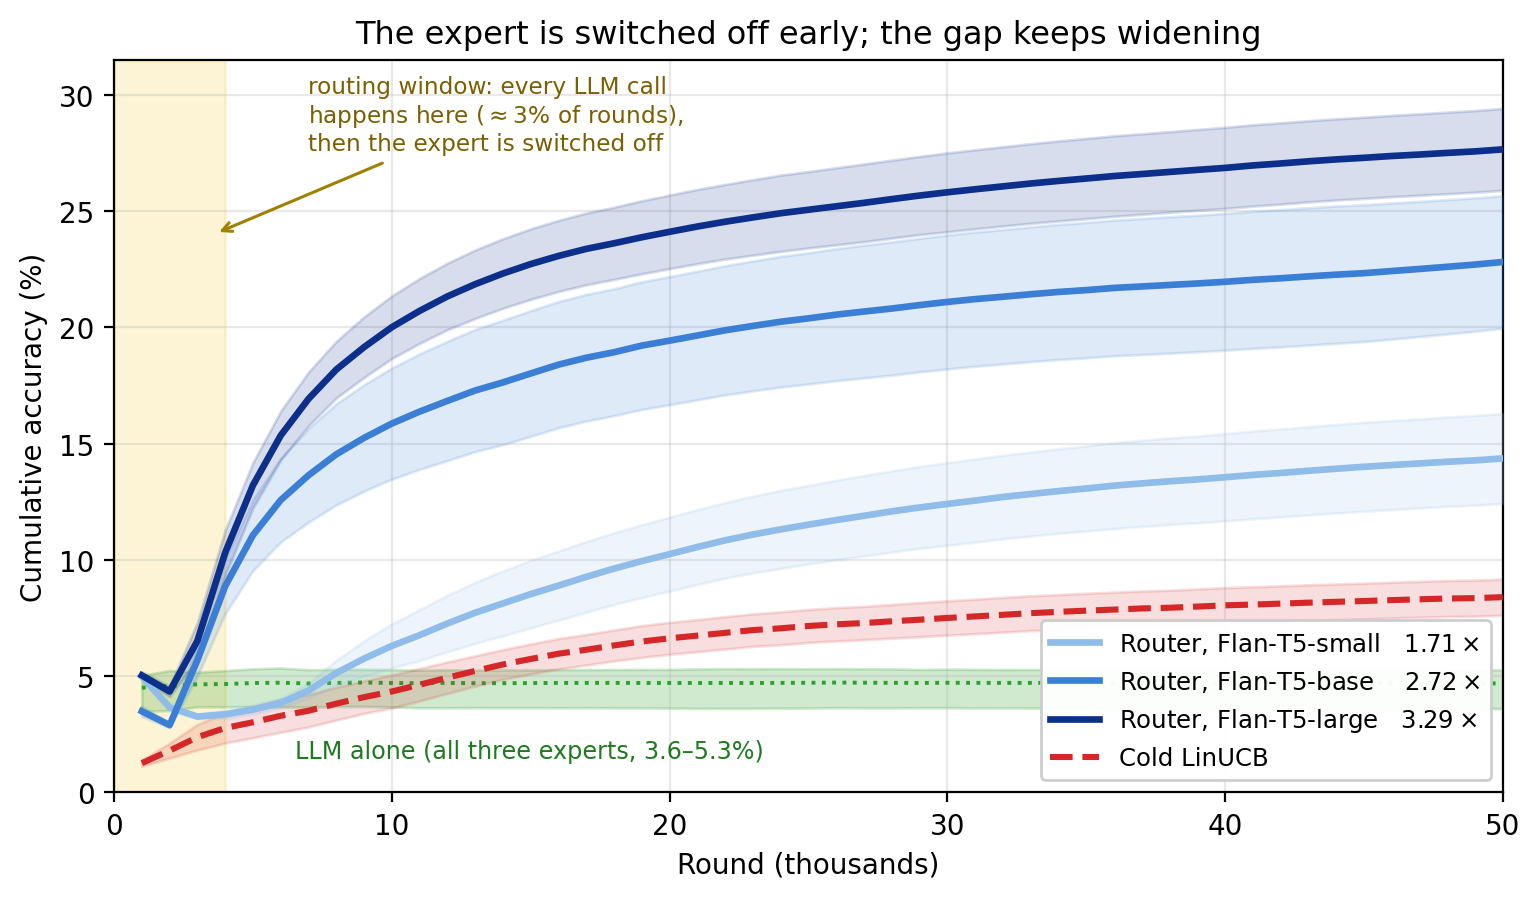
\includegraphics[width=0.78\linewidth]{multiplication.png}
\caption{Learning dynamics on AmazonCat-13K (BERT-768d, $c=100$). The Router
with Flan-T5-large (blue) pulls away from cold LinUCB (red dashed) after
roughly $t=10{,}000$ and reaches $2.34\times$ its accuracy by $T=50{,}000$. The
LLM alone (green dotted) stays at $5.3\%$.}
\label{fig:amazon-dynamics}
\end{figure}

\textbf{The multiplying configuration.} Flan-T5-large reaches $25.91\%$
against cold LinUCB's $11.05\%$ with only $3.4\%$ of rounds routed to the LLM
overall; routing is concentrated in the first $\sim5{,}000$ rounds
($33.7\%$ there). This is the shape Theorem~\ref{prop:decomp} predicts for
a positive case: $A_\tau$ is negative (the expert is $5\%$ accurate while the
learner will reach $26\%$) and small in absolute terms because $\tau$ is
small; $V_\tau$ is large; and $B_\tau$ is large because the expert stays at
$5\%$. Figure~\ref{fig:amazon-dynamics} shows the same accounting in time: at
$t=5{,}000$ the Router ($3.0\%$) and cold LinUCB ($2.1\%$) are within a point
of each other, the Router still paying acquisition regret and not yet cashing
the width reduction; at $t=10{,}000$ they stand at $4.2\%$ and $3.5\%$; and
between $10{,}000$ and $15{,}000$ the Router jumps to $12.7\%$ while cold LinUCB
reaches $6.4\%$, a gap that keeps widening to $T$.

\textbf{Equal accuracy, unequal information.} Flan-T5-small and base have the
same held-out accuracy as large to within two points, hence the same
acquisition regret, and yet deliver $1.01\times$ and $0.94\times$. Under
Theorem~\ref{prop:decomp} the only place the three can differ is
$V_\tau$, that is, in which directions their proposals cover. This is the
experimental counterpart of the distinction between policy value and
information value in Section~\ref{sec:canonical}: two experts with the same
$A_\tau$ can have very different $V_\tau$. \todo{The $\widehat\Phi$ columns
of Table~\ref{tab:diagnostics} are the direct test: the prediction is that
$\widehat\Phi(\lambda I)-\widehat\Phi(\lambda I+(\tau/n)\widehat M_{\Exp})$ is
markedly larger for large than for small/base. If it is not, the explanation
above is wrong and should be replaced.}

\textbf{BGE-1024d.} Cold LinUCB alone reaches $39.01\%$, far above every Qwen
expert. With unit-norm BGE features the expert width $u^{(1)}=1/\sqrt c=0.1$
is permanently below $u^{(0)}\ge1/\sqrt\lambda=3.16$ at $c=100$, so the Router
defers to the LLM on every round and equals it. This is a hyperparameter
failure of the Router, not evidence about $V_\tau$; \todo{add a $c$-sweep at
small $c$ (e.g.\ $c\in\{0.01,0.1,1\}$) showing the Router recovering LinUCB's
$39\%$, as promised in the rebuttal.} What the pre-runtime statistics do say
is that in BGE space cold LinUCB transfers information between arms well
($\widehat{\bar\alpha}=0.31$, so $\rho_{\lambda I}$ is bounded away from zero
across most pairs by Lemma~\ref{lem:transfer}), so widths collapse quickly on
their own and there is little left for a warm start to remove.

\paragraph{Summary across configurations.}
Twelve configurations span two datasets, two model families (60M to 7B), two
embedding spaces, and three orders of magnitude in $c$. The one configuration
that multiplies is the one where (i)~cold LinUCB leaves many directions
unresolved for a long time (high effective rank, near-orthogonal features in
BERT space), (ii)~the expert is cheap to run for a short prefix and remains
poor on the tail, and (iii)~the expert's proposals, unlike those of two
equally accurate smaller models, cover the unresolved directions. Every other
configuration fails at least one of the three, and in each case the failing
term of Theorem~\ref{prop:decomp} can be named. The deterministic Router
differs from the randomized CORRAL master of \cite{agarwal2017corralling} and
the CORRAL-style routing of \cite{chen2024llmdecision} only in how it chooses
the routed rounds; both feed every observation to the bandit learner, so the
decomposition applies to both. \todo{Add the CORRAL-routing and
offline-warm-start baselines requested in review; the decomposition predicts
that any router with the same routed set and the same observation feed has
the same $V_\tau$, so differences should appear in $A_\tau$ only.}


\section{Conclusion}
\label{sec:conclusion}

Reward multiplication in LLM--bandit hybrids is an accounting statement: the
hybrid beats cold LinUCB by the expert's direct advantage plus the value of the
data it leaves behind, and beats the expert by the learner's tail advantage.
The data-value term is governed by whether the routed actions push the
confidence widths of dangerous competitors below their gaps; the
determinant-ratio term that controls $\sqrt T$-rates cannot produce more than
a constant factor. The canonical separating instance exhibits the data-value
term in its purest form, offline, and exhibits none of it online, because
there every useful observation costs a constant amount of regret. When the
directions that trap cold LinUCB recur and the expert has a cheaper way of
covering them, an online handoff multiplies, and the multiplier is the ratio
of the two prices; when any one of recurrence, cheapness, correct targeting,
or late suboptimality of the expert is removed, it does not. This
separates the information value of an expert from its policy value and
explains why experts of equal accuracy can differ by a factor of two in what
they deliver. The pre-runtime estimates of Section~\ref{sec:diagnostics} are
the practical output: they can be computed from a labeled held-out sample
and the expert's proposals on it, before any LLM call is spent on the live
trajectory.

\paragraph{Limitations.}
The theory assumes linear reward. Theorem~\ref{thm:handoff} is an upper bound
on the hybrid and, when combined with the cold-start upper bound, does not by
itself lower-bound the gain; the positive statement about multiplication is
Proposition~\ref{prop:three-way} (offline), and the negative statement is
Proposition~\ref{prop:one-pass}; Theorem~\ref{thm:price} supplies an online
instance with a provable multiplier, but it is a constructed instance with a
fixed confidence radius and a regularization scaled to the dimension, and we
have not shown that the price ratio governs the multiplier on general
instances beyond the necessary condition of Lemma~\ref{lem:no-free-coverage}.
The constants in the catalog are not optimized and the lower bound on cold
LinUCB's regret there counts only the rounds that optimism forces. The pre-runtime estimates require a labeled held-out sample and the
expert's proposals on it; their thresholds are provisional and were not tuned
across datasets. The extension of the width-based analysis to other
confidence-based learners (OFUL, SupLinUCB, Thompson sampling) is immediate
for Lemmas~\ref{lem:loewner} and~\ref{lem:transfer}, which are statements
about design matrices, but Lemma~\ref{lem:width-limited} uses the optimistic
selection rule and would need an analogue for posterior sampling. Only two
real datasets are used; multi-expert behaviour is not stress-tested;
LLM-guided recommendation can inherit biases from pretrained models and
logged data.

\paragraph{Broader impact.}
The work is foundational theory and pre-runtime estimation for contextual
bandits. A positive impact is reducing unnecessary LLM inference in
sequential decision systems by identifying when cold-start LinUCB suffices,
which lowers compute cost and energy use. A potential negative impact is that
LLM-guided contextual-bandit systems deployed in recommendation or ranking
may inherit biases from pretrained models or logged data without auditing;
concrete harms depend on follow-on applications not studied here.

%% NOTE: the related-work patch cites four keys that must be added to
%% references.bib (BibTeX entries provided in the accompanying report):
%% graves1997asymptotically, lattimore2017end, rakhlin2013online,
%% cutkosky2022leveraging.
\bibliography{references}
\bibliographystyle{abbrv}


\appendix

\section{Related Work}\label{sec:related}
This appendix expands on the related-work discussion deferred from the
introduction. We cover (i) linear contextual bandits and confidence geometry,
(ii) model selection and expert aggregation, (iii) warm starts and prior
information, (iv) the geometry of information gain in linear bandits, and
(v) large language models for sequential decision making.

Sequential decision making with contextual information has been studied
extensively in the contextual bandit literature, where the learner must
balance exploration and exploitation under partial feedback
\cite{langford2007epoch,agarwal2014taming,foster2021statistical,
lattimore2020bandit}. In the linear setting, algorithms such as LinUCB and
OFUL achieve regret bounds that depend explicitly on the geometry of the
accumulated design matrix through self-normalized confidence ellipsoids
\cite{chu2011contextual,abbasi2011improved}. Subsequent work has developed
statistically efficient contextual bandit algorithms under general function
approximation assumptions \cite{agarwal2012contextual,foster2018practical,
foster2020beyond,simchi2022bypassing,zhu2022contextual,rucker2023infinite,
zhang2024efficient}. A central insight of this line of work is that the
conditioning of the covariance matrix determines how quickly uncertainty
shrinks and therefore how rapidly regret decreases. Our work builds on this
perspective by showing that actions selected by a frozen predictor can
reshape this geometry early in learning and accelerate subsequent adaptation.

\paragraph{Model selection and expert aggregation in bandits.}
A closely related direction studies how to combine multiple candidate
policies or base algorithms online. Classical expert-learning methods provide
regret guarantees relative to the best fixed expert in hindsight
\cite{auer2002nonstochastic}. In the bandit setting, CORRAL
\cite{agarwal2017corralling} uses Online Mirror Descent with a log-barrier
regularizer to achieve regret competitive with the best base algorithm;
subsequent refinements tighten the rates and extend the framework to
contextual and stochastic settings
\cite{pacchiano2020model,marinov2021pareto,zhu2022pareto,zhu2022near,
dann2024data}. These approaches are inherently \emph{randomized} and target
robustness: the master performs nearly as well as the best base algorithm
regardless of which one that is. Our objective is different---we want a
\emph{deterministic} rule that exploits the complementarity between a good
early frozen policy and a strong asymptotic adaptive learner to
\emph{strictly outperform} both. Correspondingly, our analysis does not
bound a relative regret against the best base, but instead tracks how early
actions selected by one policy reshape the design matrix and accelerate the
statistical efficiency of another.

\paragraph{Warm starts and prior information in contextual bandits.}
Several works have investigated how prior information can be incorporated
into contextual bandit algorithms through initialization, offline datasets,
or pretrained predictors. Such approaches can substantially improve
short-horizon performance by reducing uncertainty before online interaction
begins \cite{bastani2021mostly,zhang2019warm}. Related directions in
transfer learning and structured bandits further show that leveraging
information across tasks or user populations can accelerate adaptation and
reduce exploration requirements \cite{lazaric2012transfer,gentile2014online}.
Meta-learning approaches similarly learn priors that enable faster
exploration in new environments \cite{sharaf2019meta}. Empirical work on
neural-linear bandit architectures also demonstrates that representation
pretraining can significantly improve early decision quality
\cite{riquelme2018deep}. Our analysis formalizes these intuitions in a
linear bandit framework: informative early actions contract the confidence
ellipsoid on specific competitors (Lemmas~\ref{lem:loewner}
and~\ref{lem:transfer}), and the resulting saving is a difference of
width-limited regrets rather than an improvement of the
determinant-ratio rate, which Theorem~\ref{thm:handoff} shows cannot by
itself exceed a constant factor.

\paragraph{Geometry of information gain in linear bandits.}
A central theme in the analysis of linear bandit algorithms is that learning
efficiency is governed by the geometry of the accumulated design matrix.
Early work on stochastic linear optimization under bandit feedback showed
that regret depends explicitly on the growth of the covariance matrix
associated with the chosen actions and the resulting confidence ellipsoid
\cite{dani2008stochastic}. Subsequent analyses of linearly parameterized
bandits further clarified how the eigenvalue structure of this matrix
determines parameter identifiability and sample complexity
\cite{rusmevichientong2010linearly}. Later work established sharp
self-normalized confidence bounds and finite-time regret guarantees
expressed directly in terms of the design matrix and its inverse
\cite{abbasi2011improved}, while related results connected spectral growth
of the covariance matrix to optimal arm identification in linear settings
\cite{soare2014best}. From an information-theoretic perspective, regret can
also be related to determinant growth and effective dimension of the
covariance operator \cite{srinivas2012information,valko2013finite}. The
price \eqref{eq:price} is the single-direction shadow of the allocation
programs behind asymptotic instance-dependent lower bounds, where regret is
minimized subject to coverage constraints on every direction
\cite{graves1997asymptotically,lattimore2017end}; our use of it is
non-asymptotic and comparative: two policies on the same instance pay
different prices for the same coverage. Prior side information has also been
analyzed as hints or predictable sequences in online learning
\cite{rakhlin2013online,cutkosky2022leveraging}; there the benefit enters
through reduced loss variation, here through the design matrix. Our
work extends this geometric viewpoint by showing that a fixed policy can
shape the spectrum of the design matrix during early rounds of interaction,
thereby improving conditioning of the confidence ellipsoid and accelerating
the learning rate of subsequent adaptive exploration.

\paragraph{Large language models for sequential decision making.}
Recent work has explored the use of large language models (LLMs) as policies
in contextual bandit environments, demonstrating that frozen pretrained
models can achieve strong short-horizon performance even without online
updates \cite{chen2024llmdecision}. More broadly, LLMs exhibit strong
in-context learning capabilities \cite{brown2020language,xie2021explanation,
garg2022can,akyurek2022learning}, and instruction tuning further improves
their effectiveness in downstream decision tasks
\cite{ouyang2022training,chung2024scaling}. Several recent approaches
interpret sequential decision making itself as a sequence-modeling problem
and adapt transformer architectures to interactive settings
\cite{chen2021decision,zheng2022online,reid2022can,sun2023smart,
raparthy2023generalization,lee2023supervised}.
Closest to our work is the approach of \cite{chen2024llmdecision}, who
combine an LLM policy with an adaptive contextual bandit learner using an
online model-selection master and empirically document the
reward-multiplication phenomenon on large-scale recommendation datasets.
Our contribution relative to that line is theoretical: we give a
regret-based explanation for why such combinations can beat both components,
and replace the randomized CORRAL-style master with a deterministic
confidence-gated rule whose routing decision directly exposes the geometric
warm-start mechanism. A concurrent line of work \cite{huangcontextual} also
uses LLM uncertainty to gate exploration, but does so by calibrating an
embedding-based uncertainty estimate to adjust UCB-style exploration
bonuses, rather than by comparing self-normalized confidence radii of a
frozen predictor and an online learner; their analysis focuses on regret
improvement for a single calibrated agent, whereas we give an exact
decomposition of the hybrid's advantage, prove when its terms can be large
at once, and identify the multiplier on our positive instance as a ratio of
acquisition prices. Additional evidence that LLMs can
exhibit in-context reinforcement learning behavior
\cite{monea2024llms,krishnamurthy2024can} and that LLM-derived priors can
jump-start exploration \cite{alamdari2024jumpstarting,abbasiyadkori2024believe}
further motivates the study of principled mechanisms for combining frozen
predictors with online learners.


\section{Proofs}
\label{app:proofs}

Section~\ref{app:proof-decomp} proves the decomposition identity.
Section~\ref{app:proof-three-way} reproduces the proof of
Proposition~\ref{prop:three-way} from the original construction.
Section~\ref{app:proof-one-pass} proves Proposition~\ref{prop:one-pass}.
Sections~\ref{app:proof-width}--\ref{app:proof-transfer} prove the three
lemmas of Section~\ref{sec:width}, and Section~\ref{app:proof-handoff}
proves Theorem~\ref{thm:handoff}.

\subsection{Proof of Theorem~\ref{prop:decomp}}
\label{app:proof-decomp}

\begin{proof}
Split $[T]$ into $[1,\tau]$ and $[\tau+1,T]$. On $[1,\tau]$ the hybrid plays
$a_t^{\Exp}$, so $R_{[1,\tau]}(\Hyb_\tau)=R_{[1,\tau]}(\Exp)$. Hence
\[
R_T(\Cold)-R_T(\Hyb_\tau)
=\bigl(R_{[1,\tau]}(\Cold)-R_{[1,\tau]}(\Exp)\bigr)
+\bigl(R_{[\tau+1,T]}(\Cold)-R_{[\tau+1,T]}(\Hyb_\tau)\bigr)
=A_\tau+V_\tau ,
\]
and
\[
R_T(\Exp)-R_T(\Hyb_\tau)
=\bigl(R_{[1,\tau]}(\Exp)-R_{[1,\tau]}(\Exp)\bigr)
+\bigl(R_{[\tau+1,T]}(\Exp)-R_{[\tau+1,T]}(\Hyb_\tau)\bigr)
=B_\tau .
\]
Both are identities between sums of gaps, so they hold for every noise
realization and therefore in expectation. The ``if and only if'' statements
are restatements of the identities.
\end{proof}

\subsection{Proof of Proposition~\ref{prop:three-way}}
\label{app:proof-three-way}

We first record the standard subgaussian concentration lemma used in the
high-probability part of the argument, and then construct the linear bandit
instance and verify the three claims of Proposition~\ref{prop:three-way}.

\begin{lemma}[Subgaussian concentration, Corollary 5.5 of \cite{lattimore2020bandit}]
\label{lem:subgaussian}
Assume that $X_1-\mu,\dots,X_n-\mu$ are independent, $\sigma$-subgaussian random variables. Then for any $\varepsilon \ge 0$,
\[
\mathbb{P}\!\left(\hat{\mu} \ge \mu+\varepsilon\right)
\le
\exp\!\left(-\frac{n\varepsilon^2}{2\sigma^2}\right),
\qquad
\mathbb{P}\!\left(\hat{\mu} \le \mu-\varepsilon\right)
\le
\exp\!\left(-\frac{n\varepsilon^2}{2\sigma^2}\right),
\]
where
\[
\hat{\mu}=\frac{1}{n}\sum_{t=1}^n X_t.
\]
\end{lemma}

\subparagraph{Problem setup.}
Let the dimension satisfy $d \ge n+1$, where $n$ is the horizon. The unknown parameter is
\[
\theta^\star = e_1 \in \mathbb{R}^d,
\]
where $\{e_i\}_{i=1}^d$ denotes the standard basis. Rewards follow the stochastic linear model
\[
X_t = \langle \theta^\star, A_t \rangle + \eta_t,
\]
where $\eta_t$ are independent mean-zero $\sigma$-subgaussian random variables.

At each round $t=1,\dots,n$, the learner is offered two actions,
\[
g:=e_1,
\qquad
b_t:=L e_{t+1},
\]
where $L>1$ is a fixed constant. Their expected rewards are
\[
\langle \theta^\star,g\rangle = 1,
\qquad
\langle \theta^\star,b_t\rangle = 0.
\]
Both LinUCB variants below use the rule
\[
\mathrm{UCB}_t(a)
=
a^\top \hat{\theta}_{t-1}
+
\beta \|a\|_{V_{t-1}^{-1}},
\]
with
\[
V_{t-1}=V_0+\sum_{s<t} A_sA_s^\top,
\qquad
\hat{\theta}_{t-1}
=
V_{t-1}^{-1}\sum_{s<t} A_s X_s.
\]

\subparagraph{Algorithm 1: a constant policy.}
Consider a policy $\pi_{\mathrm{const}}$ that selects an action by maximizing $\langle \hat{\theta}_{\mathrm{const}}, a\rangle$ for some fixed parameter estimate $\hat{\theta}_{\mathrm{const}}\in\mathbb{R}^d$ that is never updated. For concreteness, take
\[
\hat{\theta}_{\mathrm{const}}
=
\frac{1}{L}\sum_{j=2}^{n+1} e_j,
\]
so that
\[
\langle \hat{\theta}_{\mathrm{const}},g\rangle = 0,
\qquad
\langle \hat{\theta}_{\mathrm{const}},b_t\rangle = 1
\quad\text{for every } t\le n.
\]
Then $\pi_{\mathrm{const}}$ selects $b_t$ at every round $t$. Since each pull of $b_t$ yields expected reward $0$ while $g$ has expected reward $1$, the cumulative pseudo-regret of $\pi_{\mathrm{const}}$ on the horizon $n$ is exactly $n$. This proves part (1) of Proposition~\ref{prop:three-way}.

The failure mode is structural rather than statistical: $\pi_{\mathrm{const}}$ never queries direction $e_1$, so no amount of data can refine $\hat{\theta}_{\mathrm{const}}$ in the reward-relevant direction. The policy has no learning mechanism. We will see, however, that the trajectory it produces is precisely what suppresses the misplaced optimism of LinUCB in the bad directions.

\subparagraph{Algorithm 2: LinUCB with isotropic initialization.}
The first LinUCB variant uses
\[
V_0=\lambda I_d,
\qquad
\hat{\theta}_0=0.
\]
At $t=1$,
\[
\|g\|_{V_0^{-1}}^2=\frac{1}{\lambda},
\qquad
\|b_1\|_{V_0^{-1}}^2=\frac{L^2}{\lambda}.
\]
Since $\hat{\theta}_0=0$, we have
\[
\mathrm{UCB}_1(b_1)>\mathrm{UCB}_1(g),
\]
so the algorithm selects $b_1$.

Now suppose inductively that the algorithm has selected $b_1,\dots,b_{t-1}$ in the first $t-1$ rounds. Then
\[
V_{t-1}
=
\lambda I_d+\sum_{s=1}^{t-1} b_s b_s^\top
=
\lambda I_d + L^2\sum_{j=2}^{t} e_j e_j^\top.
\]
Hence $V_{t-1}$ is diagonal in the standard basis. In particular, for the fresh direction $e_{t+1}$,
\[
e_{t+1}^\top V_{t-1}^{-1} e_{t+1}=\frac{1}{\lambda},
\qquad
\|b_t\|_{V_{t-1}^{-1}}^2=\frac{L^2}{\lambda},
\qquad
\|g\|_{V_{t-1}^{-1}}^2=\frac{1}{\lambda}.
\]

The key point is that although the observed rewards on $b_1,\dots,b_{t-1}$ contain noise, the estimate
\[
\hat{\theta}_{t-1}
=
V_{t-1}^{-1}\sum_{s=1}^{t-1} b_s X_s
\]
lies entirely in $\mathrm{span}\{e_2,\dots,e_t\}$. Therefore,
\[
g^\top \hat{\theta}_{t-1}=0,
\qquad
b_t^\top \hat{\theta}_{t-1}=0,
\]
because both $g=e_1$ and the fresh arm $b_t=L e_{t+1}$ are orthogonal to $\mathrm{span}\{e_2,\dots,e_t\}$.

Thus, even in the stochastic-reward setting, the comparison between $g$ and $b_t$ is determined purely by the confidence terms:
\[
\mathrm{UCB}_t(g)=\frac{\beta}{\sqrt{\lambda}},
\qquad
\mathrm{UCB}_t(b_t)=\frac{\beta L}{\sqrt{\lambda}}.
\]
Since $L>1$, we have $\mathrm{UCB}_t(b_t)>\mathrm{UCB}_t(g)$ for all $t\le n$. Hence the isotropically initialized algorithm selects $b_t$ at every round and, like $\pi_{\mathrm{const}}$, incurs cumulative pseudo-regret $n$. This proves part (2) of Proposition~\ref{prop:three-way}.

\subparagraph{Algorithm 3: LinUCB with an anisotropic warm start.}
We now define an initialization that is realized by exactly the trajectory $\pi_{\mathrm{const}}$ would produce. Fix an integer $m\ge 1$, and let
\[
V_0'
=
\lambda I_d + mL^2 \sum_{j=2}^{n+1} e_j e_j^\top,
\qquad
\hat{\theta}_0'=0.
\]
This corresponds to having observed each bad direction $L e_j$, $j=2,\dots,n+1$, exactly $m$ times before the online interaction begins --- precisely the kind of data $\pi_{\mathrm{const}}$ generates if rolled out for $mn$ rounds on a sequence of action sets containing each bad direction. Thus $V_0'$ is a genuine design matrix obtainable from a collection of outer products produced by a constant logging policy.

At $t=1$,
\[
\|g\|_{(V_0')^{-1}}^2=\frac{1}{\lambda},
\qquad
\|b_1\|_{(V_0')^{-1}}^2
=
L^2\cdot \frac{1}{\lambda+mL^2}
=
\frac{L^2}{\lambda+mL^2}.
\]
Hence, if
\[
m > \frac{\lambda(L^2-1)}{L^2},
\]
then $\frac{1}{\lambda}>\frac{L^2}{\lambda+mL^2}$, and therefore
\[
\mathrm{UCB}_1'(g)>\mathrm{UCB}_1'(b_1).
\]
So the warm-started algorithm selects $g$ at round $1$.

Suppose now that the algorithm continues to select $g$ for the first $s$ rounds. Then
\[
V_s'
=
\lambda I_d
+
mL^2 \sum_{j=2}^{n+1} e_j e_j^\top
+
s\, e_1 e_1^\top.
\]
Since each reward observed on $g$ has mean $1$,
\[
\sum_{i=1}^s X_i = s + \sum_{i=1}^s \eta_i,
\]
and therefore
\[
g^\top \hat{\theta}_s'
=
e_1^\top (V_s')^{-1}\sum_{i=1}^s g X_i
=
\frac{1}{\lambda+s}\sum_{i=1}^s X_i.
\]
Applying Lemma~\ref{lem:subgaussian} with $\mu=1$, we obtain that with probability at least $1-\delta$, simultaneously for all $1\le s\le n$,
\[
\frac{1}{s}\sum_{i=1}^s X_i
\ge
1-\sqrt{\frac{2\sigma^2\log(2n/\delta)}{s}}.
\]
On this event,
\[
g^\top \hat{\theta}_s'
\ge
\frac{s}{\lambda+s}
\left(
1-\sqrt{\frac{2\sigma^2\log(2n/\delta)}{s}}
\right).
\]

For every fresh bad arm $b_{s+1}=Le_{s+2}$,
\[
b_{s+1}^\top \hat{\theta}_s' = 0,
\]
since the online trajectory has only sampled the direction $e_1$, and the warm-start contributes only to the design matrix, not to the response vector. Moreover,
\[
\|b_{s+1}\|_{(V_s')^{-1}}^2
=
\frac{L^2}{\lambda+mL^2},
\qquad
\|g\|_{(V_s')^{-1}}^2
=
\frac{1}{\lambda+s}.
\]

On the same high-probability event,
\[
\mathrm{UCB}_{s+1}'(g)
\ge
\frac{s}{\lambda+s}
\left(
1-\sqrt{\frac{2\sigma^2\log(2n/\delta)}{s}}
\right)
+
\frac{\beta}{\sqrt{\lambda+s}},
\]
while
\[
\mathrm{UCB}_{s+1}'(b_{s+1})
=
\frac{\beta L}{\sqrt{\lambda+mL^2}}.
\]
Consequently, if $m$ is chosen large enough so that for every $1\le s\le n$,
\begin{equation}
\label{eq:m-condition}
\frac{s}{\lambda+s}
\left(
1-\sqrt{\frac{2\sigma^2\log(2n/\delta)}{s}}
\right)
+
\frac{\beta}{\sqrt{\lambda+s}}
>
\frac{\beta L}{\sqrt{\lambda+mL^2}},
\end{equation}
then, with probability at least $1-\delta$, the warm-started algorithm selects $g$ at every round, and the cumulative pseudo-regret over the $n$ online rounds is $0$ on this event. This proves part (3) of Proposition~\ref{prop:three-way}; condition~\eqref{eq:m-condition} is the explicit ``$m$ sufficiently large'' requirement referenced in the proposition statement. The condition is satisfiable by a finite $m$ whenever the left-hand side is positive for every $s$, which holds for any $\beta\ge\sigma\sqrt{2\log(2n/\delta)}$ (in particular for the radius of \cite{abbasi2011improved}), since then $\beta/\sqrt{\lambda+s}\ge\sigma\sqrt{2\log(2n/\delta)}\,\sqrt s/(\lambda+s)$.\hfill$\square$


\begin{remark}
The warm-started algorithm in the proof uses $\widehat\theta_0'=0$, i.e., it
carries the offline Gram matrix but not the offline response sum. Because
every offline observation is of an arm with expected reward $0$, the offline
response sum has mean zero in each bad direction and carrying it would only
add a mean-zero perturbation to $\widehat\theta$ in directions orthogonal to
$g$; the comparison between $g$ and $b_{s+1}$ is unchanged up to the noise
term already absorbed in the choice of $m$. We keep the convention of the
original construction.
\end{remark}

\subsection{Proof of Proposition~\ref{prop:one-pass}}
\label{app:proof-one-pass}

\begin{proof}
Work on the instance of Section~\ref{app:proof-three-way} with horizon $T$:
$\theta^\star=e_1$, $\mathcal A_t=\{g,b_t\}$ with $g=e_1$ and
$b_t=Le_{t+1}$. Fix an arbitrary expert $\Exp$ and a handoff time $\tau$.
Whatever the expert plays during rounds $1,\dots,\tau$, and whatever LinUCB
plays afterwards, the set of arms played before round $t$ is contained in
$\{g\}\cup\{b_s:s<t\}$, all of which are orthogonal to $e_{t+1}$. Hence for
every $t$, the design matrix $V_t=\lambda I+\sum_{s<t}x_{s,A_s}x_{s,A_s}^\top$
is block diagonal with the block on $e_{t+1}$ equal to $\lambda$, and
$\widehat\theta_t=V_t^{-1}b_t$ lies in $\mathrm{span}\{e_1,\dots,e_t\}$. Therefore
\[
\|b_t\|_{V_t^{-1}}^2=\frac{L^2}{\lambda},\qquad \langle\widehat\theta_t,b_t\rangle=0,
\qquad\text{for every }t\text{ and every trajectory.}
\]
So $\mathrm{UCB}_t(b_t)=\beta L/\sqrt\lambda$ exactly, for all $t$.

Now bound $\mathrm{UCB}_t(g)$. Let $s_t$ be the number of pulls of $g$ before
round $t$ and $X_1,\dots,X_{s_t}$ the rewards observed on those pulls; since
$V_t$ is diagonal with entry $\lambda+s_t$ on $e_1$ and the rewards on bad
arms enter $b_t$ only in directions orthogonal to $e_1$,
\[
\langle\widehat\theta_t,g\rangle=\frac{1}{\lambda+s_t}\sum_{i=1}^{s_t}X_i,
\qquad
\|g\|_{V_t^{-1}}^2=\frac{1}{\lambda+s_t}\le\frac1\lambda .
\]
By Lemma~\ref{lem:subgaussian} and a union bound over $s\in\{1,\dots,T\}$,
with probability at least $1-\delta$ we have
$\sum_{i\le s}X_i\le s+\sqrt{2\sigma^2s\log(2T/\delta)}$ for all $s\le T$
simultaneously. On that event,
\[
\langle\widehat\theta_t,g\rangle
\le\frac{s_t}{\lambda+s_t}+\frac{\sqrt{2\sigma^2s_t\log(2T/\delta)}}{\lambda+s_t}
\le 1+\frac{\sigma\sqrt{2\log(2T/\delta)}}{\sqrt{\lambda+s_t}}
\le 1+\kappa ,
\]
using $\sqrt{s_t}/(\lambda+s_t)\le1/\sqrt{\lambda+s_t}\le1/\sqrt\lambda$.
Hence $\mathrm{UCB}_t(g)\le1+\kappa+\beta/\sqrt\lambda$. Under the hypothesis
$\beta(L-1)/\sqrt\lambda>1+\kappa$ this is strictly less than
$\beta L/\sqrt\lambda=\mathrm{UCB}_t(b_t)$, so LinUCB, whenever it acts, plays
$b_t$. The argument did not use anything about rounds $1,\dots,\tau$ beyond
the fact that they cannot produce coverage of $e_{t+1}$ for $t>\tau$, so it
holds for every expert and every $\tau$. Since $\Delta_{t,b_t}=1$,
$R_{[\tau+1,T]}(\Hyb_\tau)=T-\tau$. Cold LinUCB plays $b_t$ on every round by
part~(2) of Proposition~\ref{prop:three-way} (no condition on $\beta$ is
needed there because $\widehat\theta_t\perp g$ on its own trajectory), so
$R_{[\tau+1,T]}(\Cold)=T-\tau$ and $V_\tau=0$.
\end{proof}

\subsection{Proof of Lemma~\ref{lem:width-limited}}
\label{app:proof-width}

\begin{proof}
Fix a round $t$ at which LinUCB acts, and write $x^\star=x_{t,a_t^\star}$,
$x=x_{t,A_t}$, $\wid(u)=\|u\|_{V_t^{-1}}$. On $\mathcal E_\delta$, Cauchy--Schwarz
gives $|\langle\widehat\theta_t-\theta^\star,u\rangle|\le\beta_t\wid(u)$ for
every $u$. By the selection rule,
$\langle\widehat\theta_t,x\rangle+\beta_t\wid(x)\ge\langle\widehat\theta_t,x^\star\rangle+\beta_t\wid(x^\star)\ge\langle\theta^\star,x^\star\rangle$,
and $\langle\widehat\theta_t,x\rangle\le\langle\theta^\star,x\rangle+\beta_t\wid(x)$.
Combining, $\Delta_{t,A_t}=\langle\theta^\star,x^\star-x\rangle\le2\beta_t\wid(x)$.
Thus $\Delta_{t,A_t}=\min\{\Delta_{t,A_t},2\beta_t\wid(x_{t,A_t})\}\le\max_a\min\{\Delta_{t,a},2\beta_t\wid(x_{t,a})\}=\Phi_t(V_t)$.
Monotonicity: $V\preceq V'$ implies $V'^{-1}\preceq V^{-1}$, so every width is
non-increasing and so is each term in the maximum.
\end{proof}

\subsection{Proof of Lemma~\ref{lem:loewner}}
\label{app:proof-loewner}

\begin{proof}
$\lambda I+M\succeq\lambda I$ gives $(\lambda I+M)^{-1}\preceq(\lambda I)^{-1}$,
which is the first claim. For the second, $\lambda I+M\succeq\lambda I+mP$, so
$x^\top(\lambda I+M)^{-1}x\le x^\top(\lambda I+mP)^{-1}x$, and for
$x\in\mathrm{Im}(P)$ the right-hand side is $\|x\|_2^2/(\lambda+m)$ because
$(\lambda I+mP)^{-1}$ acts as $(\lambda+m)^{-1}$ on $\mathrm{Im}(P)$. For the
third, if $x\perp\mathrm{Im}(M)$ then $x$ is an eigenvector of $\lambda I+M$
with eigenvalue $\lambda$, so $x^\top(\lambda I+M)^{-1}x=\|x\|_2^2/\lambda$.
\end{proof}

\subsection{Proof of Lemma~\ref{lem:transfer}}
\label{app:proof-transfer}

\begin{proof}
By the Sherman--Morrison formula,
$(V+xx^\top)^{-1}=V^{-1}-\dfrac{V^{-1}xx^\top V^{-1}}{1+x^\top V^{-1}x}$. Multiplying
on both sides by $z$,
\[
z^\top(V+xx^\top)^{-1}z
= z^\top V^{-1}z-\frac{(z^\top V^{-1}x)^2}{1+\|x\|^2_{V^{-1}}}
=\|z\|^2_{V^{-1}}\Bigl(1-\frac{(z^\top V^{-1}x)^2}{(1+\|x\|^2_{V^{-1}})\|z\|^2_{V^{-1}}}\Bigr).
\]
The bracket is at least $1-\dfrac{\|x\|^2_{V^{-1}}\|z\|^2_{V^{-1}}}{(1+\|x\|^2_{V^{-1}})\|z\|^2_{V^{-1}}}>0$
by Cauchy--Schwarz in the $V^{-1}$ inner product, so $\rho_V\in[0,1)$. At
$V=\lambda I$, $z^\top V^{-1}x=\langle z,x\rangle/\lambda$,
$\|x\|^2_{V^{-1}}=\|x\|_2^2/\lambda$, $\|z\|^2_{V^{-1}}=\|z\|_2^2/\lambda$, and
substituting gives
$\rho_{\lambda I}(x,z)=\dfrac{\langle x,z\rangle^2}{\|x\|_2^2\|z\|_2^2}\cdot\dfrac{\|x\|_2^2}{\lambda+\|x\|_2^2}$.
\end{proof}

\subsection{Proof of Theorem~\ref{thm:handoff}}
\label{app:proof-handoff}

\begin{proof}
The acquisition term is the definition of $R_{[1,\tau]}(\Hyb_\tau)=R_{[1,\tau]}(\Exp)$.
For the LinUCB phase we give two bounds and take the minimum.

\emph{First bound.} By Lemma~\ref{lem:width-limited} applied at each
$t>\tau$, $\sum_{t>\tau}\Delta_{t,A_t}\le\sum_{t>\tau}\Phi_t(V_t)$.

\emph{Second bound.} From the proof of Lemma~\ref{lem:width-limited},
$\Delta_{t,A_t}\le2\beta_t\|x_{t,A_t}\|_{V_t^{-1}}\le2\beta_T\|x_{t,A_t}\|_{V_t^{-1}}$
for $t>\tau$ (the radius $\beta_t$ is non-decreasing in $t$). Cauchy--Schwarz
over $t=\tau+1,\dots,T$ gives
\[
\sum_{t>\tau}\Delta_{t,A_t}\le2\beta_T\sqrt{(T-\tau)\sum_{t>\tau}\|x_{t,A_t}\|^2_{V_t^{-1}}} .
\]
By the elliptical potential lemma \cite[Lemma~11]{abbasi2011improved},
$\sum_{t>\tau}\min\{1,\|x_{t,A_t}\|^2_{V_t^{-1}}\}\le2\log\det V_{T+1}/\det V_{\tau+1}$;
since $\|x_{t,A_t}\|^2_{V_t^{-1}}\le L^2/\lambda$, the truncation at $1$ costs at
most a factor $\max\{1,L^2/\lambda\}$ on the sum of squares, which is the
factor $\max\{1,L/\sqrt\lambda\}$ in \eqref{eq:handoff-bound} after the square
root; with $L^2\le\lambda$ nothing is lost. This gives
the second term of \eqref{eq:handoff-bound}.

\emph{Determinant ratio.} Let $V_{\tau+1}=\sum_j\sigma_ju_ju_j^\top$ be an
eigendecomposition and $G=\sum_{t>\tau}x_{t,A_t}x_{t,A_t}^\top$. Then
$\det(V_{\tau+1}+G)/\det V_{\tau+1}=\det(I+V_{\tau+1}^{-1/2}GV_{\tau+1}^{-1/2})\le\prod_j(1+u_j^\top Gu_j/\sigma_j)$
by Hadamard's inequality for positive definite matrices, and
$u_j^\top Gu_j=\sum_{t>\tau}\langle u_j,x_{t,A_t}\rangle^2\le L^2(T-\tau)$.
Taking logarithms gives the stated bound. If all played actions lie in an
$r$-dimensional subspace $\mathrm{Im}(P)$ then $G$ is supported there and only
the $r$ eigenvalues of $V_{\tau+1}$ restricted to $\mathrm{Im}(P)$ appear, which
is how the factor $r$ in the remark after the theorem arises; if in addition
$V_{\tau+1}\succeq(\lambda+\nu\tau)P$ on that subspace, each $\sigma_j\ge\lambda+\nu\tau$.

The cold bound is the case $\tau=0$, $V_1=\lambda I$, $\sigma_j=\lambda$. The
ratio $\Psi$ in the text is the quotient of the two isotropic bounds and is
stated only to show that it does not tend to zero.
\end{proof}

\begin{remark}[Validity of the confidence event with an online warm start]
The hybrid's LinUCB phase uses $(V_{\tau+1},b_{\tau+1})$ built from the
expert-routed rounds together with the observed rewards on those rounds. The
self-normalized bound of \cite{abbasi2011improved} applies to any sequence of
(feature, reward) pairs in which the feature at round $s$ is measurable with
respect to the history before $s$, whoever chose it, so the event
$\mathcal E_\delta$ covers the hybrid's trajectory. If instead the warm start
carried $M_\tau$ but dropped $c_\tau$ (``passive'' updates), the estimate
$\widehat\theta_t$ would be biased toward zero in the directions of $M_\tau$
and the event would not be guaranteed; the Router in our experiments updates
both, and Algorithm~\ref{alg:confidence-gated} reflects this.
\end{remark}

\section{Proofs for the Catalog of Section~\ref{sec:catalog}}
\label{app:catalog}

Throughout this appendix the conventions \eqref{eq:conventions} are in force,
$\alpha:=1-\eps$, $m_0:=\lfloor\lambda/30\rfloor$, and ``LinUCB acts at round
$t$'' means that the action at $t$ is chosen by the LinUCB rule (every round
for $\Cold$; rounds $t>\tau$ for $\Hyb_\tau$). Ties in the LinUCB rule are
broken arbitrarily; every comparison we use is strict. For a policy $\pi$ and
a round $t$ we write $s(t)$, $m_j(t)$, $n_j(t)$ for the numbers of pulls of
$g$, $b$ in direction $e_j$, and $p$ in direction $e_j$ before round $t$
(all of them counted from the start, including expert-routed rounds), and we
drop the argument $t$ when no confusion arises. In the variant of
Proposition~\ref{prop:cat-gap} the roles of $g$ and $p$ are played by
$g_\eta$ and $p_{t,\eta}$ and $\alpha:=(1-\eps)\eta$; we prove everything for
general $\eta\in(0,1]$ and set $\eta=1$ outside that proposition.

\subsection{Events and their probabilities}

\begin{lemma}[Good events]
\label{lem:cat-events}
Fix a policy $\pi$ on any instance of the template. Let
$\mathcal E_{\mathrm{conf}}(\pi)$ be the event that
$\|\widehat\theta_t-\theta^\star\|_{V_t}\le\beta$ for every $t\in[T]$, where
$(V_t,b_t)$ are formed from all of $\pi$'s data before $t$. Let
$\mathcal E_{\mathrm{noise}}(\pi)$ be the event that for every direction
$j\in\{2,\dots,d\}$ and every $m\in[T]$, the sum $S_j^{(m)}$ of the noises on
the first $m$ pulls of $b$ in direction $e_j$ by $\pi$ satisfies
$|S_j^{(m)}|\le\sigma\sqrt{2m\ell_1}$. Then
$\Prb(\mathcal E_{\mathrm{conf}}(\pi))\ge1-\delta$ and
$\Prb(\mathcal E_{\mathrm{noise}}(\pi))\ge1-\delta$. Moreover, under
\eqref{eq:conventions}, $\beta\ge4\sigma\sqrt{2\ell_1}$.
\end{lemma}

\begin{proof}
All arm vectors of the template have Euclidean norm at most $L$: $\|g_\eta\|=\eta\le1$,
$\|b_t\|=L$, $\|p_{t,\eta}\|^2=\alpha^2+c^2\le2\le L^2$. Also $\|\theta^\star\|=1$.
By Theorem~2 of \cite{abbasi2011improved}, with probability at least
$1-\delta$, simultaneously for all $t$,
$\|\widehat\theta_t-\theta^\star\|_{V_t}\le\sigma\sqrt{2\log\bigl(\det(V_t)^{1/2}\det(\lambda I)^{-1/2}/\delta\bigr)}+\sqrt\lambda$.
Since $V_t\preceq(\lambda+tL^2)I$, $\det(V_t)^{1/2}\det(\lambda I)^{-1/2}\le(1+tL^2/\lambda)^{d/2}$,
so the radius is at most
$\sigma\sqrt{d\log(1+TL^2/\lambda)+2\log(1/\delta)}+\sqrt\lambda\le\sigma\sqrt{d\,\ell_0}+\sqrt\lambda\le2\sqrt\lambda=\beta$,
using $\lambda\ge1$ and $\lambda\ge\sigma^2d\ell_0$. This proves the first claim.
The theorem of \cite{abbasi2011improved} only requires the noise to be
conditionally sub-Gaussian given the past and the current action, which holds
in the reward-table model, and it applies to the data of any policy, not only
to LinUCB's own.

For the second claim, in the reward-table model the noises on successive pulls
of $b$ in direction $e_j$ form an i.i.d.\ $\sigma$-sub-Gaussian sequence
$(\eta_{j,i})_{i\ge1}$ regardless of the policy, and $S_j^{(m)}=\sum_{i\le m}\eta_{j,i}$.
By Hoeffding's inequality for sub-Gaussian sums,
$\Prb(|S_j^{(m)}|>\sigma\sqrt{2m\ell_1})\le2e^{-\ell_1}=\delta/(dT)$. A union
bound over $d-1<d$ directions and $T$ values of $m$ gives probability at most
$\delta$ for the complement. Finally $\beta=2\sqrt\lambda\ge2\sqrt{8\sigma^2\ell_1}=4\sigma\sqrt{2\ell_1}$.
\end{proof}

\begin{lemma}[Confidence consequences]
\label{lem:cat-conf}
On $\mathcal E_{\mathrm{conf}}(\pi)$, for every $t$ and every $x\in\R^d$,
$|\langle\widehat\theta_t-\theta^\star,x\rangle|\le\beta\|x\|_{V_t^{-1}}$.
Hence the index $U_t(x):=\langle\widehat\theta_t,x\rangle+\beta\|x\|_{V_t^{-1}}$
satisfies $\mu(x)\le U_t(x)\le\mu(x)+2\beta\|x\|_{V_t^{-1}}$, where
$\mu(x)=\langle\theta^\star,x\rangle$.
\end{lemma}

\begin{proof}
Cauchy--Schwarz in the $V_t$ inner product:
$|\langle\widehat\theta_t-\theta^\star,x\rangle|\le\|\widehat\theta_t-\theta^\star\|_{V_t}\|x\|_{V_t^{-1}}\le\beta\|x\|_{V_t^{-1}}$.
\end{proof}

\subsection{The state of LinUCB on the template}

Every action vector of the template is $g_\eta$, some $b$ in direction $e_j$,
or some $p_\eta$ in direction $e_j$, and the probe is the only one that couples
two coordinates. The design matrix therefore has an arrowhead structure whose
inverse is explicit.

\begin{lemma}[Arrowhead inverse]
\label{lem:arrowhead}
Let $V=\lambda I+Se_1e_1^\top+\sum_{j=2}^{d}\bigl(M_je_je_j^\top+n_jq_jq_j^\top\bigr)$
with $S,M_j,n_j\ge0$ and $q_j=\alpha e_1+ce_j$. Put
\[
D_j:=\lambda+M_j+n_jc^2,\qquad u_j:=\alpha cn_j,
\]
\[
Q:=\lambda+S+\alpha^2\sum_{j\ge2}n_j-\sum_{j\ge2}\frac{u_j^2}{D_j}
=\lambda+S+\alpha^2\sum_{j\ge2}\frac{n_j(\lambda+M_j)}{D_j}.
\]
Then $Q\ge\lambda$ and
\begin{align*}
(V^{-1})_{11}&=\frac1Q,&
(V^{-1})_{1j}&=-\frac{u_j}{D_jQ},\\
(V^{-1})_{jj}&=\frac1{D_j}+\frac{u_j^2}{D_j^2Q},&
(V^{-1})_{jj'}&=\frac{u_ju_{j'}}{D_jD_{j'}Q}\ \ (j\ne j'),
\end{align*}
for $j,j'\ge2$. In particular, if $n_j=0$ then
$(V^{-1})_{jj}=1/D_j$ and $(V^{-1})_{1j}=(V^{-1})_{jj'}=0$ for all $j'\ne j$; and
if $n_j\ge1$ and $M_j\ge1$ then $(V^{-1})_{jj}\le 1/D_j+1/M_j$.
\end{lemma}

\begin{proof}
Write $V=\begin{pmatrix}a&u^\top\\ u&D\end{pmatrix}$ with
$a=\lambda+S+\alpha^2\sum_jn_j$, $u=(u_2,\dots,u_d)^\top$, and
$D=\mathrm{diag}(D_2,\dots,D_d)$; this is the matrix in the statement because
$q_jq_j^\top=\alpha^2e_1e_1^\top+\alpha c(e_1e_j^\top+e_je_1^\top)+c^2e_je_j^\top$.
The Schur complement of $D$ is $a-u^\top D^{-1}u=Q$, and the block inverse
formula gives
$(V^{-1})_{11}=Q^{-1}$, $(V^{-1})_{1,\cdot}=-Q^{-1}u^\top D^{-1}$, and
$(V^{-1})_{\cdot,\cdot}=D^{-1}+D^{-1}uu^\top D^{-1}Q^{-1}$ on the lower block,
which are the displayed entries. The second expression for $Q$ follows from
$\alpha^2n_j-u_j^2/D_j=\alpha^2n_j(D_j-c^2n_j)/D_j=\alpha^2n_j(\lambda+M_j)/D_j$,
and it shows $Q\ge\lambda$. If $n_j=0$ then $u_j=0$ and the special case
follows. For the last claim, $Q\ge\alpha^2n_j(\lambda+M_j)/D_j\ge\alpha^2n_jM_j/D_j$,
so $u_j^2/(D_j^2Q)\le\alpha^2c^2n_j^2D_j/(D_j^2\alpha^2n_jM_j)=c^2n_j/(D_jM_j)\le1/M_j$,
using $c^2n_j\le D_j$.
\end{proof}

\begin{lemma}[State of a policy on the template]
\label{lem:cat-state}
Let $\pi$ be any policy on an instance of the template and $t$ a round. Then
$V_t$ is the matrix of Lemma~\ref{lem:arrowhead} with $S=\eta^2s$, $M_j=m_jL^2$,
$n_j$ the probe counts, and $q_j=p_\eta$'s direction vector. For a direction
$j\ge2$ with $n_j=0$:
\begin{enumerate}[itemsep=1pt,topsep=1pt,leftmargin=*]
\item[(a)] $\|e_j\|^2_{V_t^{-1}}=1/(\lambda+m_jL^2)$ and
$\widehat\theta_{t,j}=LS_j^{(m_j)}/(\lambda+m_jL^2)$, where $S_j^{(m_j)}$ is the
sum of the noises on the $m_j$ pulls of $b$ in direction $e_j$;
\item[(b)] $\|g_\eta\|^2_{V_t^{-1}}=\eta^2/Q\le1/\lambda$ and
$\|p_\eta\|^2_{V_t^{-1}}=\alpha^2/Q+c^2/(\lambda+m_jL^2)\le2/\lambda$ for the probe
in direction $e_j$.
\end{enumerate}
For any direction with $m_j\ge1$, $\|e_j\|^2_{V_t^{-1}}\le2/(m_jL^2)$.
\end{lemma}

\begin{proof}
The form of $V_t$ is immediate from the definitions. For (a), Lemma~\ref{lem:arrowhead}
with $n_j=0$ gives $(V_t^{-1})_{jj}=1/D_j=1/(\lambda+m_jL^2)$ and that the $j$-th
row of $V_t^{-1}$ vanishes off the diagonal. The $j$-th coordinate of the
response vector $b_t$ is $L\sum r$ over the pulls of $b$ in direction $e_j$
plus $c\sum r$ over the pulls of $p$ in that direction; the second sum is
empty, and since $\mu(b)=0$ the first is $LS_j^{(m_j)}$. Hence
$\widehat\theta_{t,j}=(V_t^{-1})_{jj}LS_j^{(m_j)}$. For (b),
$\|g_\eta\|^2_{V_t^{-1}}=\eta^2(V_t^{-1})_{11}=\eta^2/Q$ and
$\|p_\eta\|^2_{V_t^{-1}}=\alpha^2(V_t^{-1})_{11}+2\alpha c(V_t^{-1})_{1j}+c^2(V_t^{-1})_{jj}
=\alpha^2/Q+c^2/D_j$, using $(V_t^{-1})_{1j}=0$; both bounds use $Q\ge\lambda$,
$D_j\ge\lambda$, $\alpha\le1$, $c\le1$, $\eta\le1$. The last claim is the last
claim of Lemma~\ref{lem:arrowhead} with $M_j=m_jL^2\ge L^2\ge1$ together with
$1/D_j\le1/(m_jL^2)$, and it holds trivially when $n_j=0$.
\end{proof}

\subsection{Three reusable facts}

\begin{lemma}[Optimism trap]
\label{lem:cat-trap}
Let $\pi$ be a policy on an instance of the template and suppose LinUCB acts
for $\pi$ at round $t$. On $\mathcal E_{\mathrm{conf}}(\pi)\cap\mathcal E_{\mathrm{noise}}(\pi)$,
if the direction $j=j(t)$ satisfies $n_j(t)=0$ and $m_j(t)<m_0$, then
\[
U_t(b_t)\ \ge\ \tfrac34\,\frac{\beta L}{\sqrt{\lambda+m_j(t)L^2}}\ >\ \max\{U_t(g_\eta),U_t(p_{t,\eta})\},
\]
where the probe term is omitted if the probe is not offered at $t$. In
particular LinUCB plays $b_t$.
\end{lemma}

\begin{proof}
Write $m=m_j(t)$ and $D=\lambda+mL^2$. By Lemma~\ref{lem:cat-state}(a),
$U_t(b_t)=L\widehat\theta_{t,j}+\beta L\|e_j\|_{V_t^{-1}}=L^2S_j^{(m)}/D+\beta L/\sqrt D$.
On $\mathcal E_{\mathrm{noise}}$, $|L^2S_j^{(m)}/D|\le L^2\sigma\sqrt{2m\ell_1}/D\le L\sigma\sqrt{2\ell_1}/\sqrt D$,
since $L\sqrt m\le\sqrt D$; by Lemma~\ref{lem:cat-events} this is at most
$(\beta/4)L/\sqrt D$. This gives the first inequality. For the second, by
Lemma~\ref{lem:cat-conf} and Lemma~\ref{lem:cat-state}(b),
$U_t(g_\eta)\le\eta+2\beta\eta/\sqrt Q\le1+2\beta/\sqrt\lambda$ and
$U_t(p_{t,\eta})\le(1-\eps)\eta+2\beta\sqrt{2/\lambda}\le1+2\sqrt2\,\beta/\sqrt\lambda$.
Since $\beta=2\sqrt\lambda$, $1\le\beta/(2\sqrt\lambda)$, so both indices are at
most $(\tfrac12+2\sqrt2)\beta/\sqrt\lambda$. It remains to check
$\tfrac34L/\sqrt D>(\tfrac12+2\sqrt2)/\sqrt\lambda$, i.e.\
$D<\lambda L^2\,(3/4)^2/(\tfrac12+2\sqrt2)^2$. Numerically
$(3/4)^2/(\tfrac12+2\sqrt2)^2=0.5625/11.0784>0.0507$. Since $m\le m_0-1<\lambda/30$,
$D<\lambda+\lambda L^2/30=\lambda L^2(1/L^2+1/30)\le\lambda L^2(1/64+1/30)<0.0491\,\lambda L^2$,
using $L\ge8$. The inequality holds with room to spare.
\end{proof}

\begin{lemma}[Bad-pull cap]
\label{lem:cat-cap}
Let $\pi$ be a policy on an instance of the template. On
$\mathcal E_{\mathrm{conf}}(\pi)$, at any round $t$ at which LinUCB acts for
$\pi$ and plays $b_t$ with direction $j$, $m_j(t)\le8\beta^2/\eta^2$; if
moreover $n_j(t)=0$, then $m_j(t)\le4\beta^2/\eta^2$. Consequently the number
of rounds at which LinUCB acting for $\pi$ plays $b$ in direction $e_j$ is at
most $8\beta^2/\eta^2+1$, and at most $4\beta^2/\eta^2+1$ if no probe in
direction $e_j$ is ever played by $\pi$.
\end{lemma}

\begin{proof}
By Lemma~\ref{lem:width-limited}, a bad arm with gap $\eta$ is played only if
$\eta\le2\beta L\|e_j\|_{V_t^{-1}}$, i.e.\ $\|e_j\|^2_{V_t^{-1}}\ge\eta^2/(4\beta^2L^2)$.
If $m_j(t)\ge1$, Lemma~\ref{lem:cat-state} gives $\|e_j\|^2_{V_t^{-1}}\le2/(m_j(t)L^2)$,
so $m_j(t)\le8\beta^2/\eta^2$; with $n_j(t)=0$ the sharper bound
$\|e_j\|^2_{V_t^{-1}}=1/(\lambda+m_j(t)L^2)\le1/(m_j(t)L^2)$ gives $m_j(t)\le4\beta^2/\eta^2$.
Since $m_j(\cdot)$ increases by one at each such round, the number of rounds
at which $b$ in direction $e_j$ is played with $m_j(t)\le M$ is at most $M+1$.
\end{proof}

\begin{lemma}[Expert routing]
\label{lem:expert-routes}
Let $\eps L<c$ and let $\Exp_w$ be the frozen linear policy with
$\widehat\theta_{\Exp}=e_1+w\sum_{j\ge2}e_j$ on the instance with $g_\eta,b_t,p_{t,\eta}$.
\begin{enumerate}[itemsep=1pt,topsep=1pt,leftmargin=*]
\item[(a)] If $w\in(\eta/L,(1-\eps)\eta/(L-c))$, a nonempty interval, then
$\Exp_w$ plays $p_{t,\eta}$ whenever the probe is offered and $b_t$ otherwise.
\item[(b)] If $w\in(\eps\eta/c,\eta/L)$, a nonempty interval, then $\Exp_w$ plays
$p_{t,\eta}$ whenever the probe is offered and $g_\eta$ otherwise.
\end{enumerate}
All three comparisons are strict.
\end{lemma}

\begin{proof}
The scores are $\langle\widehat\theta_{\Exp},g_\eta\rangle=\eta$,
$\langle\widehat\theta_{\Exp},b_t\rangle=wL$, and
$\langle\widehat\theta_{\Exp},p_{t,\eta}\rangle=(1-\eps)\eta+wc$. The probe beats
$g_\eta$ iff $wc>\eps\eta$ and beats $b_t$ iff $w<(1-\eps)\eta/(L-c)$; $b_t$
beats $g_\eta$ iff $w>\eta/L$. The interval in (a) is nonempty iff
$(1-\eps)\eta L>\eta(L-c)$, i.e.\ $c>\eps L$, and every $w$ in it satisfies
$w>\eta/L>\eps\eta/c$ because $c>\eps L$. The interval in (b) is nonempty iff
$\eps\eta/c<\eta/L$, again $c>\eps L$; for $w$ in it, $w<\eta/L<(1-\eps)\eta/(L-c)$.
\end{proof}

\begin{lemma}[Widths at handoff after $n$ probes in each direction]
\label{lem:cat-handoff}
Let $V=\lambda I+n\sum_{j=2}^{K+1}q_jq_j^\top$ with $q_j=\alpha e_1+ce_j$, $\alpha>0$,
$n\ge1$. Then for every $j\in\{2,\dots,K+1\}$,
\[
\|e_j\|^2_{V^{-1}}\ \le\ \frac1{nc^2}+\frac1{K\lambda},
\qquad\text{and}\qquad
Q=\lambda+\frac{\alpha^2Kn\lambda}{\lambda+nc^2}\ \ge\ \lambda\Bigl(1+\frac{\alpha^2K}{2c^2}\Bigr)\ \text{ if } nc^2\ge\lambda .
\]
\end{lemma}

\begin{proof}
Apply Lemma~\ref{lem:arrowhead} with $S=0$, $M_j=0$, $n_j=n$: $D_j=D:=\lambda+nc^2$,
$u_j=\alpha cn$, and $Q=\lambda+\alpha^2Kn\lambda/D$. Then
$(V^{-1})_{jj}=1/D+(\alpha cn)^2/(D^2Q)$. The first term is at most $1/(nc^2)$.
For the second, $Q\ge\alpha^2Kn\lambda/D$, so
$(\alpha cn)^2/(D^2Q)\le(\alpha cn)^2D/(D^2\alpha^2Kn\lambda)=c^2n/(DK\lambda)\le1/(K\lambda)$,
using $c^2n\le D$. The bound on $Q$ follows from $D\le2nc^2$ when $nc^2\ge\lambda$.
\end{proof}

\subsection{Proof of Lemma~\ref{lem:no-free-coverage}}

Fix $u$. At a round $t\in I$ with $\langle x_{t,\pi_t},u\rangle=0$ the
contribution to the coverage is zero. At a round with
$\langle x_{t,\pi_t},u\rangle\ne0$, the definition \eqref{eq:price} gives
$\Delta_{t,\pi_t}/\langle x_{t,\pi_t},u\rangle^2\ge\pi_t(u)\ge\pi(u)$, i.e.\
$\langle x_{t,\pi_t},u\rangle^2\le\Delta_{t,\pi_t}/\pi(u)$ (if $\pi(u)=0$ the bound
is vacuous). Summing over $I$ gives the first claim. For the second, let
$u$ be a unit vector and $V=V_{\tau+1}=\lambda I+M_\tau$. By Cauchy--Schwarz in
the $V$ inner product,
$1=(u^\top u)^2=(u^\top V^{1/2}V^{-1/2}u)^2\le(u^\top Vu)(u^\top V^{-1}u)$, so
$\|u\|^2_{V^{-1}}\ge1/(\lambda+u^\top M_\tau u)$, and
$u^\top M_\tau u=\sum_{t\le\tau}\langle x_{t,A_t},u\rangle^2\le R_{[1,\tau]}(\Exp)/\pi(u)$
by the first claim applied to the expert on $[1,\tau]$. \qed

\subsection{Proof of Theorem~\ref{thm:price}}

We work on $\mathcal E_{\mathrm{conf}}(\Cold)\cap\mathcal E_{\mathrm{noise}}(\Cold)\cap\mathcal E_{\mathrm{conf}}(\Hyb_{\tau_0})$,
which has probability at least $1-3\delta$ by Lemma~\ref{lem:cat-events}. Set
$\eta=1$.

\paragraph{(i) The expert.}
By Lemma~\ref{lem:expert-routes}(a), $\Exp_w$ plays $p_t$ at every $t\le\tau_0$
(gap $\eps$) and $b_t$ at every $t>\tau_0$ (gap $1$), so $R_T(\Exp)=\eps Kn+(T-Kn)$.

\paragraph{(ii) Cold LinUCB, lower bound.}
We claim that at every round $t\in[T]$ with $m_{j(t)}(t)<m_0$, cold LinUCB
plays $b_t$. We argue by induction on $t$. Suppose the claim holds for all
rounds before $t$ and let $j=j(t)$ with $m_j(t)<m_0$. If cold LinUCB had
played the probe in direction $e_j$ at some earlier round $t'$ (so $j(t')=j$),
then $m_j(t')\le m_j(t)<m_0$ and the claim at $t'$ says it played $b_{t'}$,
a contradiction; hence $n_j(t)=0$. Lemma~\ref{lem:cat-trap} now gives that
LinUCB plays $b_t$. (The base case $t=1$ is the same argument with no earlier
rounds.) Direction $e_j$ is offered at exactly $n$ rounds in $[1,Kn]$, and at
each of the first $\min\{n,m_0\}$ of them $m_j<m_0$, so cold LinUCB plays the
bad arm, paying $1$ each time. With $n\ge m_0$ this gives $R_{[1,Kn]}(\Cold)\ge Km_0$,
and $A_{\tau_0}=R_{[1,Kn]}(\Cold)-R_{[1,Kn]}(\Exp)\ge Km_0-\eps Kn$ by (i).

\paragraph{(iii) Cold LinUCB, upper bound.}
Cold LinUCB acts at every round. By Lemma~\ref{lem:cat-cap} it plays $b$ in
each of the $K$ directions at most $8\beta^2+1$ times over the horizon, each
costing $1$. Probes exist only at rounds $t\le Kn$ and cost $\eps$ each, so
probe pulls cost at most $\eps Kn$. Pulls of $g$ cost nothing. Hence
$R_T(\Cold)\le K(8\beta^2+1)+\eps Kn$.

\paragraph{(iv) The hybrid.}
During $t\le\tau_0$ the hybrid plays the expert's actions, which by (i) are
the probes, each direction exactly $n$ times. Hence
$V_{\tau_0+1}=\lambda I+n\sum_{j=2}^{K+1}p^{(j)}p^{(j)\top}$ with $p^{(j)}=\alpha e_1+ce_j$,
and Lemma~\ref{lem:cat-handoff} gives, for every bad direction,
$\|e_j\|^2_{V_{\tau_0+1}^{-1}}\le1/(nc^2)+1/(K\lambda)$. With $nc^2\ge36\lambda L^2=9\beta^2L^2$
and $K\lambda\ge36\lambda L^2=9\beta^2L^2$ this is at most $2/(9\beta^2L^2)$, so
$2\beta L\|e_j\|_{V_{\tau_0+1}^{-1}}\le2\sqrt2/3<1$. Now fix $t>\tau_0$. The
hybrid's design matrix satisfies $V_t\succeq V_{\tau_0+1}$, so by
Lemma~\ref{lem:loewner} $\|e_{j(t)}\|_{V_t^{-1}}\le\|e_{j(t)}\|_{V_{\tau_0+1}^{-1}}$,
and by Lemma~\ref{lem:cat-conf}, $U_t(b_t)\le0+2\beta L\|e_{j(t)}\|_{V_t^{-1}}<1\le U_t(g)$.
Since $\mathcal A_t=\{g,b_t\}$, LinUCB plays $g$, with gap $0$. Therefore
$R_{[\tau_0+1,T]}(\Hyb_{\tau_0})=0$, $R_T(\Hyb_{\tau_0})=R_{[1,\tau_0]}(\Exp)=\eps Kn$,
$V_{\tau_0}=R_{[Kn+1,T]}(\Cold)-0\ge0$, and $B_{\tau_0}=(T-Kn)-0$.

\paragraph{The ratios.}
From (ii), (iii), (iv): $R_T(\Cold)/R_T(\Hyb_{\tau_0})\ge Km_0/(\eps Kn)=m_0/(\eps n)$
and $\le(K(8\beta^2+1)+\eps Kn)/(\eps Kn)=1+(8\beta^2+1)/(\eps n)$; the
expert ratio is (i) over (iv). At $n=\lceil36\lambda L^2/c^2\rceil$, since
$36\lambda L^2/c^2\ge36\cdot60\cdot64>1$ we have $n\le37\lambda L^2/c^2$, and
$m_0\ge\lambda/30-1\ge\lambda/60$ because $\lambda\ge60$; hence
$m_0/(\eps n)\ge(\lambda/60)c^2/(37\eps\lambda L^2)=c^2/(2220\,\eps L^2)$. For the
upper bound, $8\beta^2+1=32\lambda+1$ and $n\ge36\lambda L^2/c^2$ give
$(8\beta^2+1)/(\eps n)\le(32\lambda+1)c^2/(36\eps\lambda L^2)\le c^2/(\eps L^2)$
since $\lambda\ge1$. \qed

\subsection{Proof of Proposition~\ref{prop:cat-mimic}}

Work on $\mathcal E_{\mathrm{conf}}(\Cold)\cap\mathcal E_{\mathrm{noise}}(\Cold)$
(probability $\ge1-2\delta$). There are no probes, so $n_j\equiv0$ for every
policy.

\emph{(i)} Let $t\le Km_0$ and $j=j(t)$. Direction $e_j$ was offered at
$\lceil t/K\rceil-1\le m_0-1$ earlier rounds, so $m_j(t)\le m_0-1<m_0$ for cold
LinUCB, and Lemma~\ref{lem:cat-trap} (with the probe term absent) says cold
LinUCB plays $b_t$. Hence cold LinUCB plays $b_t$ at every $t\le Km_0$, and
so does $\Exp$. Fix $\tau\le Km_0$. The two policies $\Cold$ and $\Hyb_\tau$
play the same action vectors in the same order during $[1,\tau]$; in the
reward-table model they therefore observe the same rewards, so their states
$(V_{\tau+1},b_{\tau+1})$ coincide. From round $\tau+1$ on both run LinUCB
from that state on the same action sets and the same reward table, so they
play the same actions at every round. Thus $R_I(\Cold)=R_I(\Hyb_\tau)$ for every
interval $I$, $A_\tau=R_{[1,\tau]}(\Cold)-R_{[1,\tau]}(\Exp)=\tau-\tau=0$, and $V_\tau=0$.

\emph{(ii)} For any $\tau$, $R_T(\Hyb_\tau)\ge R_{[1,\tau]}(\Exp)=\tau$. By
Lemma~\ref{lem:cat-cap} with $n_j\equiv0$, cold LinUCB plays each bad
direction at most $4\beta^2+1$ times, so $R_T(\Cold)\le K(4\beta^2+1)=K(16\lambda+1)$.
For $\tau>Km_0$, $R_T(\Cold)/R_T(\Hyb_\tau)\le K(16\lambda+1)/(Km_0)\le(16\lambda+1)/(\lambda/60)=960+60/\lambda\le961$. \qed

\subsection{Proof of Proposition~\ref{prop:cat-tail}}

Work on the event of Theorem~\ref{thm:price}. By Lemma~\ref{lem:expert-routes}(b),
$\Exp_w$ plays every probe during $[1,\tau_0]$ and $g$ afterwards, so
$R_T(\Exp)=\eps Kn$. The hybrid's routed rounds are the same probes as in
Theorem~\ref{thm:price}(iv), so its state at handoff and its subsequent play
are identical to those established there: $R_T(\Hyb_{\tau_0})=\eps Kn$ and
$R_{[\tau_0+1,T]}(\Hyb_{\tau_0})=0$. Hence $B_{\tau_0}=0-0=0$. Cold LinUCB does not
depend on the expert, so $A_{\tau_0}$ and $V_{\tau_0}$ are as in
Theorem~\ref{thm:price}. \qed

\subsection{Proof of Proposition~\ref{prop:cat-wrong}}

Work on $\mathcal E_{\mathrm{conf}}(\Cold)\cap\mathcal E_{\mathrm{conf}}(\Hyb_{\tau_0})\cap\mathcal E_{\mathrm{noise}}(\Hyb_{\tau_0})$
(probability $\ge1-3\delta$). Here $d=2K+1$; coordinates $2,\dots,K+1$ are the
bad directions and $K+2,\dots,2K+1$ the nuisance directions. The probe $p'_t$
couples $e_1$ with a nuisance coordinate only, so Lemma~\ref{lem:arrowhead}
applies with the nuisance coordinates playing the role of the probed $j$'s
and the bad coordinates having $n_j=0$ for every policy at every round.

\emph{Cold LinUCB.} Since $n_j\equiv0$ on bad coordinates,
Lemma~\ref{lem:cat-cap} gives at most $4\beta^2+1$ bad pulls in each of the $K$
directions, costing $1$ each; probe pulls occur only at $t\le Kn$ and cost
$\eps$ each; so $R_T(\Cold)\le K(4\beta^2+1)+\eps Kn$.

\emph{The hybrid.} During $[1,\tau_0]$ it plays the $Kn$ probes, paying $\eps Kn$.
At handoff, $V_{\tau_0+1}=\lambda I+n\sum_{i}q_iq_i^\top$ over the $K$ nuisance
directions with $q_i=\alpha e_1+ce_{K+1+i}$, and the bad coordinates are
untouched: by Lemma~\ref{lem:arrowhead} (with $M_j=n_j=0$ on them),
$\|e_j\|^2_{V_{\tau_0+1}^{-1}}=1/\lambda$ for every bad direction and the estimate
has zero $j$-th coordinate. By Lemma~\ref{lem:cat-handoff} applied to the
nuisance block, $Q\ge\lambda(1+\alpha^2K/(2c^2))$ once $nc^2\ge\lambda$, which holds
since $n\ge36\lambda L^2/c^2$. As $\alpha=1-\eps\ge1-1/L\ge7/8$ and $c\le1$,
$Q\ge\lambda(1+49K/128)\ge16\lambda=4\beta^2$ because $K\ge36L^2\ge2304$. Hence at
every $t>\tau_0$, since $Q$ only grows, $U_t(g)\le1+2\beta/\sqrt Q\le2$ by
Lemma~\ref{lem:cat-conf}. On the other hand, for $t>\tau_0$ and $j=j(t)$ with
$m_j(t)=m$, Lemma~\ref{lem:cat-state}(a) and $\mathcal E_{\mathrm{noise}}(\Hyb_{\tau_0})$
give, exactly as in the proof of Lemma~\ref{lem:cat-trap},
$U_t(b_t)\ge\tfrac34\beta L/\sqrt{\lambda+mL^2}$, which exceeds $2$ as soon as
$\lambda+mL^2<\tfrac9{64}\beta^2L^2=\tfrac9{16}\lambda L^2$, i.e.\ $m<\tfrac9{16}\lambda-\lambda/L^2$.
With $L\ge8$, $\tfrac9{16}\lambda-\lambda/L^2\ge\tfrac{35}{64}\lambda>\lambda/2$, so this holds
whenever $m\le\lfloor\lambda/2\rfloor-1$. Thus at every round $t>\tau_0$ at which
$m_{j(t)}(t)<\lfloor\lambda/2\rfloor$ the hybrid plays the bad arm. Each direction
is offered at least $\lfloor(T-\tau_0)/K\rfloor\ge\lfloor\lambda/2\rfloor$ times after
$\tau_0$, so each is pulled at least $\lfloor\lambda/2\rfloor$ times, and
$R_{[\tau_0+1,T]}(\Hyb_{\tau_0})\ge K\lfloor\lambda/2\rfloor$. Hence
$R_T(\Hyb_{\tau_0})\ge\eps Kn+K\lfloor\lambda/2\rfloor$.

\emph{The ratio and $V_{\tau_0}$.} Since $\lambda\ge60$, $\lfloor\lambda/2\rfloor\ge\lambda/4$,
and for $x\ge0$, $(a+x)/(b+x)\le\max\{a/b,1\}$; with $a=K(16\lambda+1)$,
$b=K\lambda/4$, $x=\eps Kn$ this gives $R_T(\Cold)/R_T(\Hyb_{\tau_0})\le64+4/\lambda\le65$.
Finally $V_{\tau_0}=R_{[\tau_0+1,T]}(\Cold)-R_{[\tau_0+1,T]}(\Hyb_{\tau_0})\le R_{[\tau_0+1,T]}(\Cold)-K\lfloor\lambda/2\rfloor$.
The expert's Gram matrix $n\sum_iq_iq_i^\top$ has range in
$\mathrm{span}\{e_1,e_{K+2},\dots,e_{2K+1}\}$, which is orthogonal to the span of
the bad directions, so the principal angle is $90^\circ$. \qed

\subsection{Proof of Proposition~\ref{prop:cat-cheap}}

On $\mathcal E_{\mathrm{conf}}(\Cold)$, Lemma~\ref{lem:cat-cap} with $n_j\equiv0$
gives $R_T(\Cold)\le K(4\beta^2+1)=K(16\lambda+1)$; since $R_T(\pi)\ge0$ for every
$\pi$, $(R_T(\Cold)-R_T(\pi))/T\le K(16\lambda+1)/T$, and with $\lambda=\sigma^2d\ell_0$
and $d=K+1$ this is $O(\sigma^2K^2\ell_0/T)$. For the second claim, the
certificate $2\beta L\|e_j\|_{V_{\tau+1}^{-1}}<1$ means $\|e_j\|^2_{V_{\tau+1}^{-1}}<1/(4\beta^2L^2)$,
while Lemma~\ref{lem:no-free-coverage} gives
$\|e_j\|^2_{V_{\tau+1}^{-1}}\ge1/(\lambda+R_{[1,\tau]}(\Exp)/\pi(e_j))$; combining,
$R_{[1,\tau]}(\Exp)/\pi(e_j)>4\beta^2L^2-\lambda$. On the template,
$\pi(e_j)=\min\{1/L^2,\eps/c^2\}$ while probes are offered; the acquisition
regret must exceed $\pi(e_j)(4\beta^2L^2-\lambda)$ for each of the $K$ directions
that has to be certified, and the contributions of different directions come
from disjoint sets of rounds because no action vector of the template has
nonzero components on two bad directions. \qed

\subsection{Proof of Proposition~\ref{prop:cat-gap}}

The proof of Theorem~\ref{thm:price} goes through with $\eta$ carried along;
we indicate the changes. Work on the same three events. (i)~By
Lemma~\ref{lem:expert-routes}(a), $R_T(\Exp)=\eps\eta Kn+\eta(T-Kn)$.
(ii)~Lemma~\ref{lem:cat-trap} was proved for general $\eta$, and the induction
is unchanged; each forced bad pull now costs $\eta$, so
$R_{[1,Kn]}(\Cold)\ge\eta Km_0$. (iii)~Lemma~\ref{lem:cat-cap} gives at most
$8\beta^2/\eta^2+1$ bad pulls in each direction at cost $\eta$, and probe pulls
cost $\eps\eta$, so $R_T(\Cold)\le\eta K(8\beta^2/\eta^2+1)+\eps\eta Kn$.
(iv)~At handoff, Lemma~\ref{lem:cat-handoff} with $\alpha=(1-\eps)\eta>0$ gives
$\|e_j\|^2_{V_{\tau_0+1}^{-1}}\le1/(nc^2)+1/(K\lambda)\le2\eta^2/(9\beta^2L^2)$ under
$nc^2\ge9\beta^2L^2/\eta^2$ and $K\lambda\ge9\beta^2L^2/\eta^2$, i.e.\ $n\ge36\lambda L^2/(\eta^2c^2)$
and $K\ge36L^2/\eta^2$. Then $U_t(b_t)\le2\beta L\|e_j\|_{V_t^{-1}}\le(2\sqrt2/3)\eta<\eta\le U_t(g_\eta)$
for all $t>\tau_0$ by Lemmas~\ref{lem:loewner} and~\ref{lem:cat-conf}, so the
hybrid plays $g_\eta$ and $R_T(\Hyb_{\tau_0})=\eps\eta Kn$. The ratio bounds
follow: the lower bound is $\eta Km_0/(\eps\eta Kn)=m_0/(\eps n)$, and at
$n=\lceil36\lambda L^2/(\eta^2c^2)\rceil\le37\lambda L^2/(\eta^2c^2)$ this is at least
$(\lambda/60)\eta^2c^2/(37\eps\lambda L^2)=\eta^2c^2/(2220\,\eps L^2)$; the upper bound
is $1+(8\beta^2/\eta^2+1)/(\eps n)\le1+(32\lambda+\eta^2)c^2/(36\eps\lambda L^2)\le1+c^2/(\eps L^2)$. \qed

\subsection{Proof of Corollary~\ref{cor:cat-oracle}}

On the event of Proposition~\ref{prop:one-pass}, the hybrid plays $b_t$ at
every $t>\tau$, so $R_{[\tau+1,T]}(\Hyb_\tau)=T-\tau$, while the routed rounds
cost nothing because the expert plays the optimal arm; hence
$R_T(\Hyb_\tau)=T-\tau$ and $R_T(\Exp)=0$. Cold LinUCB also plays $b_t$ at
every round by Proposition~\ref{prop:one-pass} with $\tau=0$, so
$R_{[1,\tau]}(\Cold)=\tau$ and $R_{[\tau+1,T]}(\Cold)=T-\tau$. Therefore
$A_\tau=\tau-0$, $V_\tau=(T-\tau)-(T-\tau)=0$, and $B_\tau=0-(T-\tau)$. \qed

\subsection{Remarks on the constants}

The constants $36$, $30$, $65$, $961$, $2220$ come from three places: the
factor $\tfrac34$ by which noise can reduce a bad arm's index below its bonus,
the factor $\tfrac12+2\sqrt2$ by which the good arm's or the probe's index can
exceed its mean at a cold start, and the choice $\beta=2\sqrt\lambda$. None of
them is tight. What matters in Theorem~\ref{thm:price} is the structure of
\eqref{eq:price-ratio}: the lower bound is (forced cold pulls per direction)
divided by (probe cost per direction), the upper bound is (maximal cold pulls
per direction) divided by the same, and both numerators are independent of
$\eps$, $c$, and $K$. The gap between $m_0\asymp\lambda$ and $8\beta^2\asymp\lambda$
is a constant factor, and that is why the multiplier is pinned to the price
ratio up to constants. The same structure with $\eta$ gives the bounds in
Proposition~\ref{prop:cat-gap}, where the looseness is a factor $\eta^2$ rather
than a constant because the forced pulls in Lemma~\ref{lem:cat-trap} are
counted before the good arm's index has come down to its mean; a sharper
count of cold LinUCB's pulls after the good arm is well estimated, as in the
proof of Proposition~\ref{prop:cat-wrong}, would remove it, but with probes
available to cold LinUCB the required control of the estimate in a coupled
coordinate is more delicate and we have not carried it out.


\section{Confidence-Gated Meta-Algorithm: Full Description}
\label{app:meta-algorithm}

This appendix expands the brief description of
Section~\ref{sec:handoff} into the full round-by-round walkthrough,
states the deterministic confidence-gated routing rule, and provides
the pseudocode used in our experiments. The Router is the adaptive-$\tau$ version of the handoff hybrid
$\Hyb_\tau$ of Section~\ref{sec:preliminaries}: it chooses, round by round,
whether the expert or LinUCB acts, and feeds every observation to LinUCB.
Theorem~\ref{thm:handoff} applies to it with the acquisition term summed over
expert-routed rounds.

Rather than encoding prior knowledge through a single improved
initialization, we assume access to \emph{multiple frozen policy
estimators} $\{(\widehat\theta_i,V^{(i)})\}_{i=1}^m$. Each pair should
be thought of as a constant policy obtained offline:
$\widehat\theta_i$ is a fixed linear predictor and $V^{(i)}$ is the
corresponding design matrix that captures the geometry of the data on
which that predictor was trained. Our goal is not to compete with the
single best expert in hindsight, an objective closer in spirit to
online model-selection methods such as CORRAL
\cite{agarwal2017corralling,chen2024llmdecision}, which provide
robustness guarantees of the form ``perform nearly as well as the best
base algorithm.'' Here we want to collect the data-value term $V_\tau$ of
Theorem~\ref{prop:decomp} when it is available while paying as little
acquisition regret as possible, and to fall back to LinUCB otherwise.

\paragraph{Setting.}
At each round $t=1,\dots,T$, the learner observes a finite action set
$\mathcal A_t$ with feature vectors
$\{x_{t,a}\}_{a\in\mathcal A_t}\subseteq\mathbb R^d$, selects an action
$A_t\in\mathcal A_t$, and observes reward
$r_t = \langle\theta^\star,x_{t,A_t}\rangle + \eta_t$,
with $\eta_t$ conditionally mean-zero sub-Gaussian.
We are given $m$ frozen estimators
$\{(\widehat\theta_i,V^{(i)})\}_{i=1}^m$ and an online LinUCB learner
with state $(V_t,b_t,\widehat\theta_t)$, where
$\widehat\theta_t = V_t^{-1}b_t$. The frozen estimators are never
updated; only LinUCB is updated online.

\paragraph{Expert proposals and geometry-aware confidence.}
Each frozen expert $i\in[m]$ proposes the greedy action
$a_t^{(i)}\in\arg\max_{a\in\mathcal A_t}\langle\widehat\theta_i,x_{t,a}\rangle$.
To measure how trustworthy expert $i$ is on the current round, we
evaluate the uncertainty of its proposed action under its own design
geometry,
\[
u_t^{(i)} \;:=\; \bigl\|x_{t,a_t^{(i)}}\bigr\|_{(V^{(i)})^{-1}},
\qquad
\|x\|_{M^{-1}} \;:=\; \sqrt{x^\top M^{-1}x}.
\]
The interpretation is simple. If the proposed action lies in directions
that are well covered by the offline data underlying expert $i$, then
$u_t^{(i)}$ is small and the expert is more trustworthy; if the current
context points in directions poorly represented in $V^{(i)}$, then
$u_t^{(i)}$ is large and the expert should be trusted less. We treat
LinUCB itself as an additional candidate, indexed by $0$, with proposal
$a_t^{(0)}\in\arg\max_a\langle\widehat\theta_t,x_{t,a}\rangle+\alpha_t\|x_{t,a}\|_{V_t^{-1}}$
and uncertainty score $u_t^{(0)} := \|x_{t,a_t^{(0)}}\|_{V_t^{-1}}$.

\paragraph{Deterministic confidence-gated selection.}
The natural rule is to prefer the frozen expert whose proposed action
has the smallest uncertainty score, unless the online learner is
already at least as confident. Concretely, with
$i_t^\star\in\arg\min_{i\in[m]}u_t^{(i)}$,
\[
I_t \;=\;
\begin{cases}
i_t^\star, & \text{if }u_t^{(i_t^\star)}<u_t^{(0)},\\[2pt]
0, & \text{otherwise},
\end{cases}
\qquad A_t \;:=\; a_t^{(I_t)}.
\]
The master is entirely deterministic. Early in learning, LinUCB
typically has a large confidence radius, so a frozen expert may be
preferred; as data accumulate, $V_t$ grows and the LinUCB uncertainty
shrinks, and eventually the adaptive learner becomes the most confident
option and takes over automatically.

\paragraph{Optional permanent handover to LinUCB.}
To formalize the idea that LinUCB should eventually dominate, we include
a one-way switching criterion. With upper-confidence scores
$U_t^{(i)} = \langle\widehat\theta_i,x_{t,a_t^{(i)}}\rangle + \alpha_i\|x_{t,a_t^{(i)}}\|_{(V^{(i)})^{-1}}$
for each frozen expert and lower-confidence score
$L_t^{(0)} = \langle\widehat\theta_t,x_{t,a_t^{(0)}}\rangle - \alpha_t\|x_{t,a_t^{(0)}}\|_{V_t^{-1}}$
for LinUCB, if $L_t^{(0)} \ge \max_{i\in[m]} U_t^{(i)}$ for $K$
consecutive rounds we permanently hand control to LinUCB.

\begin{algorithm}[t]
\caption{Confidence-Gated Master over Frozen Policies and LinUCB}
\label{alg:confidence-gated}
\begin{algorithmic}[1]
\Require Frozen estimators $\{(\widehat{\theta}_i,V^{(i)})\}_{i=1}^m$, regularization $\lambda>0$, confidence parameters $\{\alpha_t\}_{t=1}^T$
\State Initialize LinUCB state:
\[
V_1=\lambda I_d,\qquad b_1=0,\qquad \widehat{\theta}_1=0
\]
\State Set $\textsc{handover}\gets \mathrm{False}$
\For{$t=1,\dots,T$}
    \State Observe action set $\mathcal{A}_t$
    \State Compute LinUCB proposal
    \[
    a_t^{(0)} \in \arg\max_{a\in\mathcal{A}_t}
    \left\{
    \langle \widehat{\theta}_t,x_{t,a}\rangle
    + \alpha_t \|x_{t,a}\|_{V_t^{-1}}
    \right\}
    \]
    \State Set $u_t^{(0)} \gets \|x_{t,a_t^{(0)}}\|_{V_t^{-1}}$
    \For{$i=1,\dots,m$}
        \State Compute frozen proposal
        \[
        a_t^{(i)} \in \arg\max_{a\in\mathcal{A}_t}
        \langle \widehat{\theta}_i,x_{t,a}\rangle
        \]
        \State Set $u_t^{(i)} \gets \|x_{t,a_t^{(i)}}\|_{(V^{(i)})^{-1}}$
    \EndFor
    \If{$\textsc{handover}=\mathrm{True}$}
        \State $A_t \gets a_t^{(0)}$
    \Else
        \State Choose $i_t^\star \in \arg\min_{i\in[m]} u_t^{(i)}$
        \If{$u_t^{(i_t^\star)} < u_t^{(0)}$}
            \State $A_t \gets a_t^{(i_t^\star)}$
        \Else
            \State $A_t \gets a_t^{(0)}$
        \EndIf
    \EndIf
    \State Observe reward $r_t$
    \State Update LinUCB:
    \[
    V_{t+1}\gets V_t + x_{t,A_t}x_{t,A_t}^\top,
    \qquad
    b_{t+1}\gets b_t + r_t x_{t,A_t},
    \qquad
    \widehat{\theta}_{t+1}\gets V_{t+1}^{-1}b_{t+1}
    \]
    \State Compute $U_t^{(i)}$ for all $i\in[m]$ and $L_t^{(0)}$
    \If{$L_t^{(0)} \ge \max_{i\in[m]} U_t^{(i)}$ for $K$ consecutive rounds}
        \State $\textsc{handover}\gets \mathrm{True}$
    \EndIf
\EndFor
\end{algorithmic}
\end{algorithm}

\paragraph{Distinction from randomized model selection.}
The deterministic, sample-by-sample geometric routing distinguishes
Algorithm~\ref{alg:confidence-gated} from CORRAL-style randomized
masters in two ways. First, it can exploit context-level information
about which estimator is reliable on \emph{this particular} action
set; second, because it is deterministic, the choice of which rounds to route
is a function of the current widths rather than of a sampled index. Both
rules feed the played action and the observed reward into $(V_t,b_t)$, so
both produce the online warm start $(M_\tau,c_\tau)$ whose value is
$V_\tau$ in Theorem~\ref{prop:decomp}; the decomposition itself does not
distinguish them, and any difference between them shows up in which rounds
are routed, i.e., in $A_\tau$ and in the composition of $M_\tau$.


\section{Pre-Runtime Estimates: Definitions and Consistency}
\label{app:diagnostics}

This appendix gives the formal definitions behind Section~\ref{sec:diagnostics}
and the elementary consistency statements that justify estimating them on a
held-out sample. Throughout, $\mathcal D=\{(\mathcal A_s,\{x_{s,a}\}_{a\in\mathcal A_s},\{r_{s,a}\}_{a\in\mathcal A_s})\}_{s=1}^{n}$
is a labeled held-out sample of $n$ contexts drawn from the same distribution
as the online stream, with a reward label for every candidate action (for
binary Precision@1 this is the ground-truth label), and $a_s^{\Exp}$ is the
expert's proposal on context $s$. Nothing in the online trajectory is used.

\subsection{Definitions}
\label{app:diag-defs}

\paragraph{Gap estimates.} Let $\widehat\theta_{\mathrm{or}}$ be the ridge
estimate fitted on all $(x_{s,a},r_{s,a})$ pairs of $\mathcal D$ with
regularization $\lambda$, and
$\widehat\Delta_{s,a}:=\max_{a'}\langle\widehat\theta_{\mathrm{or}},x_{s,a'}\rangle-\langle\widehat\theta_{\mathrm{or}},x_{s,a}\rangle$.
For binary reward with a single correct action one may instead use the label
directly, $\widehat\Delta_{s,a}=\ind\{a\ne a_s^\star\}$.

\paragraph{Expert Gram matrix.}
$\widehat M_{\Exp}:=\sum_{s=1}^nx_{s,a_s^{\Exp}}x_{s,a_s^{\Exp}}^\top$. For a target
number $\tau$ of routed rounds, $(\tau/n)\widehat M_{\Exp}$ is an unbiased
estimate of $\E[M_\tau]$ when the expert is followed for $\tau$ rounds on
contexts from the same distribution.

\paragraph{Width-limited regret under a design.} For a positive definite
$V$ and radius $\beta$,
\[
\widehat\Phi(V):=\frac1n\sum_{s=1}^n\max_{a\in\mathcal A_s}\min\bigl\{\widehat\Delta_{s,a},\,2\beta\|x_{s,a}\|_{V^{-1}}\bigr\}.
\]
We evaluate it at $V=\lambda I$ (cold start) and at
$V=\lambda I+(\tau/n)\widehat M_{\Exp}$ (after $\tau$ expert rounds). The
difference $\widehat\Phi(\lambda I)-\widehat\Phi(\lambda I+(\tau/n)\widehat M_{\Exp})$
is the estimated reduction, at a single future round, in the regret LinUCB
can still incur, attributable to the expert's data. It is zero whenever the
expert's proposals lie in directions orthogonal to every competitor whose
width exceeds its gap (Lemma~\ref{lem:loewner}), which is the failure mode the
principal-angle proxy detects coarsely.

\paragraph{Acquisition regret.}
$\widehat C_{\Exp}(\tau):=\tau\cdot\frac1n\sum_s\widehat\Delta_{s,a_s^{\Exp}}$.

\paragraph{Tail check.} $\widehat{\mathrm{acc}}_{\Exp}:=\frac1n\sum_s\ind\{a_s^{\Exp}=a_s^\star\}$
and $\widehat{\mathrm{acc}}_{\mathrm{or}}:=\frac1n\sum_s\ind\{\arg\max_a\langle\widehat\theta_{\mathrm{or}},x_{s,a}\rangle=a_s^\star\}$.
The learner's online accuracy is at most about $\widehat{\mathrm{acc}}_{\mathrm{or}}$
(up to the usual generalization gap), so $B_\tau>0$ requires
$\widehat{\mathrm{acc}}_{\Exp}<\widehat{\mathrm{acc}}_{\mathrm{or}}$ by a margin.

\paragraph{Net-value rule.} With $n_{\mathrm{fut}}=T-\tau$ future rounds,
\[
\widehat N(\tau):=n_{\mathrm{fut}}\bigl[\widehat\Phi(\lambda I)-\widehat\Phi(\lambda I+(\tau/n)\widehat M_{\Exp})\bigr]-\widehat C_{\Exp}(\tau).
\]
A handoff is predicted to multiply when $\widehat N(\tau)$ is a large
positive fraction of $n_{\mathrm{fut}}\widehat\Phi(\lambda I)$ for some
moderate $\tau$ and the tail check passes. We use ``large'' to mean at least
one third; this threshold is provisional. Two caveats bound what the rule
can certify. First, $\widehat\Phi(\lambda I)$ is the regret cold LinUCB could
incur at round one, not what it incurs on average over its own trajectory,
so a positive $\widehat N$ is not sufficient. Second, $\widehat N$ counts only
the saving on \emph{future} rounds and therefore misses the concurrent
channel of Theorem~\ref{prop:decomp}: on the instance of
Theorem~\ref{thm:price} the saving is carried by $A_\tau$ (cold pays for its
exploration inside the routed window at the higher price), the warm widths on
the bad arms stay near the gap, $\widehat\Phi$ barely moves, and
$\widehat N(\tau_0)<0$ even though the handoff provably multiplies. So a
negative $\widehat N$ argues against a tail-channel ($V_\tau$) multiplier but
does not exclude a concurrent-channel ($A_\tau$) one. The estimate that
covers both channels at once is a \emph{dry run}: replay the held-out
contexts (resampled to a horizon $T'$) with rewards drawn from the labels or
the ridge fit, simulate cold LinUCB and LinUCB warm-started from
$\lambda I+(\tau/n)\widehat M_{\Exp}$, and compare
$\widehat R_{T'}(\Cold)$ against
$\widehat C_{\Exp}(\tau)+\widehat R_{[\tau+1,T']}(\mathrm{warm})$. The dry run
uses no LLM calls beyond the held-out proposals already collected and no
online rounds; its cost is one bandit simulation per candidate $\tau$.

\subsection{Consistency}
\label{app:consistency}

\begin{lemma}[Concentration of the held-out quantities]
\label{lem:diag-concentration}
Suppose contexts are i.i.d.\ and $\widehat\Delta_{s,a}=\Delta_{s,a}$ (labels are
exact). Then for any fixed $V$, $\widehat\Phi(V)$ is an average of $n$ i.i.d.\
variables in $[0,\Delta_{\max}]$ with mean $\E[\Phi_t(V)]$, so
$|\widehat\Phi(V)-\E\Phi_t(V)|\le\Delta_{\max}\sqrt{\log(2/\delta)/(2n)}$ with
probability $1-\delta$ (Hoeffding); the same holds for
$\widehat C_{\Exp}(\tau)/\tau$ and for the two accuracies. For the warm design,
$\|\tfrac1n\widehat M_{\Exp}-\E[xx^\top]\|_{\mathrm{op}}\le CL^2\sqrt{\log(2d/\delta)/n}$
with probability $1-\delta$ (matrix Bernstein), and since
$V\mapsto\|x\|_{V^{-1}}$ is Lipschitz on $\{V\succeq\lambda I\}$ with constant
$\|x\|_2/(2\lambda^{3/2})$ in operator norm, $\widehat\Phi(\lambda I+(\tau/n)\widehat M_{\Exp})$
is within $O\bigl(\beta L\tau\lambda^{-3/2}L^2\sqrt{\log(2d/\delta)/n}\bigr)$ of
its population counterpart.
\end{lemma}

\begin{proof}
The scalar statements are Hoeffding's inequality applied to bounded i.i.d.\
summands; $\Phi_t(V)\in[0,\Delta_{\max}]$ because it is a maximum of minima
each bounded by a gap. The matrix statement is the matrix Bernstein inequality
for i.i.d.\ PSD summands of operator norm at most $L^2$. For the Lipschitz
claim, $\|x\|^2_{V^{-1}}-\|x\|^2_{V'^{-1}}=x^\top V^{-1}(V'-V)V'^{-1}x$, bounded by
$\|x\|_2^2\|V'-V\|_{\mathrm{op}}/\lambda^2$, and $|\sqrt u-\sqrt v|\le|u-v|/(2\sqrt{\min\{u,v\}})$
with $\min\{u,v\}\ge\|x\|_2^2/(\lambda+L^2\tau)$; the stated constant follows
after simplification. Plugging into the definition of $\widehat\Phi$ and
using that $\min\{\cdot,\cdot\}$ and $\max$ are $1$-Lipschitz completes the
proof.
\end{proof}

When labels are not exact, $\widehat\Delta$ carries the error of the ridge
fit; this affects the first argument of the minimum only and is the usual
price of a gap-dependent quantity.

\subsection{Relation to the Four Proxies}
\label{app:proxies}

The four statistics of Table~\ref{tab:diagnostics}, inherited from an earlier
version of this work, are cheaper than $\widehat\Phi$ and each bounds one
ingredient of it:
\begin{itemize}[itemsep=1pt,topsep=1pt,leftmargin=*]
\item \emph{Effective rank} $\widehat r=\mathrm{tr}(\widehat\Sigma)/\|\widehat\Sigma\|_{\mathrm{op}}$
of the context covariance. By the elliptical potential bound, cold LinUCB can
have at most $O(\widehat r\log T)$ rounds at which some played width exceeds
a fixed level, so a small $\widehat r$ means the cold-start widths, and with
them $\Phi_t(V^{\Cold}_t)$, fall quickly on their own.
\item \emph{Coherence} $\widehat{\bar\alpha}$, the median over actions of the
minimum pairwise cosine. By Lemma~\ref{lem:transfer} the cosine is the
transfer coefficient at a cold start up to the factor $\|x\|^2/(\lambda+\|x\|^2)$;
positive coherence means cold observations shrink the widths of other
arms from the first round.
\item \emph{Gap tail}, the fraction of held-out contexts whose estimated
runner-up gap is below $\eta$. Small gaps cap the first argument of the
minimum in $\Phi_t$; a heavy tail means many rounds are cheap whatever the
widths are, which by itself argues \emph{against} a large multiplier.
\item \emph{Subspace mismatch}, the largest principal angle between the
top-$\widehat r$ eigenspaces of $\widehat M_{\Exp}$ and of the context
covariance. An angle near $90^\circ$ means the expert's data covers
directions that carry little of the online context mass, so by
Lemma~\ref{lem:loewner} it cannot reduce the widths that matter. The earlier
version used this statistic inconsistently (as a deployment rule in one place
and a quality check in another); here it is only a coarse indicator that
$\widehat\Phi$ supersedes.
\end{itemize}

\section*{NeurIPS Paper Checklist}

%%% BEGIN INSTRUCTIONS %%%
The checklist is designed to encourage best practices for responsible machine learning research, addressing issues of reproducibility, transparency, research ethics, and societal impact. Do not remove the checklist: {\bf The papers not including the checklist will be desk rejected.} The checklist should follow the references and follow the (optional) supplemental material.  The checklist does NOT count towards the page
limit. 

Please read the checklist guidelines carefully for information on how to answer these questions. For each question in the checklist:
\begin{itemize}
    \item You should answer \answerYes{}, \answerNo{}, or \answerNA{}.
    \item \answerNA{} means either that the question is Not Applicable for that particular paper or the relevant information is Not Available.
    \item Please provide a short (1--2 sentence) justification right after your answer (even for \answerNA). 
   % \item {\bf The papers not including the checklist will be desk rejected.}
\end{itemize}

{\bf The checklist answers are an integral part of your paper submission.} They are visible to the reviewers, area chairs, senior area chairs, and ethics reviewers. You will also be asked to include it (after eventual revisions) with the final version of your paper, and its final version will be published with the paper.

The reviewers of your paper will be asked to use the checklist as one of the factors in their evaluation. While \answerYes{} is generally preferable to \answerNo{}, it is perfectly acceptable to answer \answerNo{} provided a proper justification is given (e.g., error bars are not reported because it would be too computationally expensive'' or ``we were unable to find the license for the dataset we used''). In general, answering \answerNo{} or \answerNA{} is not grounds for rejection. While the questions are phrased in a binary way, we acknowledge that the true answer is often more nuanced, so please just use your best judgment and write a justification to elaborate. All supporting evidence can appear either in the main paper or the supplemental material, provided in appendix. If you answer \answerYes{} to a question, in the justification please point to the section(s) where related material for the question can be found.

IMPORTANT, please:
\begin{itemize}
    \item {\bf Delete this instruction block, but keep the section heading ``NeurIPS Paper Checklist"},
    \item  {\bf Keep the checklist subsection headings, questions/answers and guidelines below.}
    \item {\bf Do not modify the questions and only use the provided macros for your answers}.
\end{itemize} 
 

%%% END INSTRUCTIONS %%%


\begin{enumerate}

\item {\bf Claims}
    \item[] Question: Do the main claims made in the abstract and introduction accurately reflect the paper's contributions and scope?
    \item[] Answer: \answerYes{} % Replace by \answerYes{}, \answerNo{}, or \answerNA{}.
    \item[] Justification: The abstract and introduction state the problem setting (LLM warm-starts in linear contextual bandits), the exact decomposition of the hybrid's advantage (Theorem~\ref{prop:decomp}), the round-level width bound that governs the data-value term (Lemma~\ref{lem:width-limited}), the offline/online contrast on the canonical instance (Propositions~\ref{prop:three-way} and~\ref{prop:one-pass}), the handoff regret bound (Theorem~\ref{thm:handoff}), and the pre-runtime estimates and experiments. Claims are stated with the scope the proofs support; items still to be computed are marked in the text.
    \item[] Guidelines:
    \begin{itemize}
        \item The answer \answerNA{} means that the abstract and introduction do not include the claims made in the paper.
        \item The abstract and/or introduction should clearly state the claims made, including the contributions made in the paper and important assumptions and limitations. A \answerNo{} or \answerNA{} answer to this question will not be perceived well by the reviewers. 
        \item The claims made should match theoretical and experimental results, and reflect how much the results can be expected to generalize to other settings. 
        \item It is fine to include aspirational goals as motivation as long as it is clear that these goals are not attained by the paper. 
    \end{itemize}

\item {\bf Limitations}
    \item[] Question: Does the paper discuss the limitations of the work performed by the authors?
    \item[] Answer: \answerYes{} % Replace by \answerYes{}, \answerNo{}, or \answerNA{}.
    \item[] Justification: Limitations are discussed at the end of Section~\ref{sec:conclusion}: linear reward, the constructed nature of the instance of Theorem~\ref{thm:price} and the unoptimized constants of the catalog, the one-sided nature of the pre-runtime estimates and their provisional thresholds, the dependence on a labeled held-out sample and on the expert's proposals, the restriction to LinUCB-style optimistic selection in Lemma~\ref{lem:width-limited}, the use of only two real datasets, and the lack of multi-expert stress tests.
    \item[] Guidelines:
    \begin{itemize}
        \item The answer \answerNA{} means that the paper has no limitation while the answer \answerNo{} means that the paper has limitations, but those are not discussed in the paper. 
        \item The authors are encouraged to create a separate ``Limitations'' section in their paper.
        \item The paper should point out any strong assumptions and how robust the results are to violations of these assumptions (e.g., independence assumptions, noiseless settings, model well-specification, asymptotic approximations only holding locally). The authors should reflect on how these assumptions might be violated in practice and what the implications would be.
        \item The authors should reflect on the scope of the claims made, e.g., if the approach was only tested on a few datasets or with a few runs. In general, empirical results often depend on implicit assumptions, which should be articulated.
        \item The authors should reflect on the factors that influence the performance of the approach. For example, a facial recognition algorithm may perform poorly when image resolution is low or images are taken in low lighting. Or a speech-to-text system might not be used reliably to provide closed captions for online lectures because it fails to handle technical jargon.
        \item The authors should discuss the computational efficiency of the proposed algorithms and how they scale with dataset size.
        \item If applicable, the authors should discuss possible limitations of their approach to address problems of privacy and fairness.
        \item While the authors might fear that complete honesty about limitations might be used by reviewers as grounds for rejection, a worse outcome might be that reviewers discover limitations that aren't acknowledged in the paper. The authors should use their best judgment and recognize that individual actions in favor of transparency play an important role in developing norms that preserve the integrity of the community. Reviewers will be specifically instructed to not penalize honesty concerning limitations.
    \end{itemize}

\item {\bf Theory assumptions and proofs}
    \item[] Question: For each theoretical result, does the paper provide the full set of assumptions and a complete (and correct) proof?
    \item[] Answer: \answerYes{} % Replace by \answerYes{}, \answerNo{}, or \answerNA{}.
    \item[] Justification: Section~\ref{sec:preliminaries} states the linear contextual-bandit setup and the three policies compared; Section~\ref{sec:catalog} states the decomposition (Theorem~\ref{prop:decomp}) and the catalog. Section~\ref{sec:width} states the confidence event under which Lemma~\ref{lem:width-limited} holds, and Lemmas~\ref{lem:loewner} and~\ref{lem:transfer} are stated as exact linear-algebra identities. Section~\ref{sec:handoff} states Theorem~\ref{thm:handoff} with the exact determinant ratio. All proofs are in Appendix~\ref{app:proofs}; the consistency statement for the held-out estimates is Lemma~\ref{lem:diag-concentration} in Appendix~\ref{app:diagnostics}.
    \item[] Guidelines:
    \begin{itemize}
        \item The answer \answerNA{} means that the paper does not include theoretical results. 
        \item All the theorems, formulas, and proofs in the paper should be numbered and cross-referenced.
        \item All assumptions should be clearly stated or referenced in the statement of any theorems.
        \item The proofs can either appear in the main paper or the supplemental material, but if they appear in the supplemental material, the authors are encouraged to provide a short proof sketch to provide intuition. 
        \item Inversely, any informal proof provided in the core of the paper should be complemented by formal proofs provided in appendix or supplemental material.
        \item Theorems and Lemmas that the proof relies upon should be properly referenced. 
    \end{itemize}

    \item {\bf Experimental result reproducibility}
    \item[] Question: Does the paper fully disclose all the information needed to reproduce the main experimental results of the paper to the extent that it affects the main claims and/or conclusions of the paper (regardless of whether the code and data are provided or not)?
    \item[] Answer: \answerYes{} % Replace by \answerYes{}, \answerNo{}, or \answerNA{}.
    \item[] Justification: Section~\ref{sec:exp-setup} specifies the datasets (OneShotWikiLinks-311 and AmazonCat-13K), baselines (Router/Algorithm~\ref{alg:confidence-gated}, LLM-only, Cold LinUCB), embedding pipelines (BERT-768d for Flan-T5, BGE-1024d for Qwen2.5), hyperparameters ($\lambda=0.1$, $\alpha_t=\max(0.1, 0.9985^t)$), confidence-parameter sweep range ($c\in\{100, 1000, 5000, 10000, 25000, 50000\}$), seed counts, and the round-level update protocol for $(V_t,b_t)$. Sections~\ref{sec:wiki} and~\ref{sec:amazon} report results for every configuration, including the WikiLinks confidence-sweep table (Table~\ref{tab:wiki-csweep}) and AmazonCat learning-dynamics figure (Figure~\ref{fig:amazon-dynamics}). The diagnostics computed pre-runtime are formally defined in Appendix~\ref{app:diagnostics}. All datasets and pretrained models used are publicly available.
    \item[] Guidelines:
    \begin{itemize}
        \item The answer \answerNA{} means that the paper does not include experiments.
        \item If the paper includes experiments, a \answerNo{} answer to this question will not be perceived well by the reviewers: Making the paper reproducible is important, regardless of whether the code and data are provided or not.
        \item If the contribution is a dataset and\slash or model, the authors should describe the steps taken to make their results reproducible or verifiable. 
        \item Depending on the contribution, reproducibility can be accomplished in various ways. For example, if the contribution is a novel architecture, describing the architecture fully might suffice, or if the contribution is a specific model and empirical evaluation, it may be necessary to either make it possible for others to replicate the model with the same dataset, or provide access to the model. In general. releasing code and data is often one good way to accomplish this, but reproducibility can also be provided via detailed instructions for how to replicate the results, access to a hosted model (e.g., in the case of a large language model), releasing of a model checkpoint, or other means that are appropriate to the research performed.
        \item While NeurIPS does not require releasing code, the conference does require all submissions to provide some reasonable avenue for reproducibility, which may depend on the nature of the contribution. For example
        \begin{enumerate}
            \item If the contribution is primarily a new algorithm, the paper should make it clear how to reproduce that algorithm.
            \item If the contribution is primarily a new model architecture, the paper should describe the architecture clearly and fully.
            \item If the contribution is a new model (e.g., a large language model), then there should either be a way to access this model for reproducing the results or a way to reproduce the model (e.g., with an open-source dataset or instructions for how to construct the dataset).
            \item We recognize that reproducibility may be tricky in some cases, in which case authors are welcome to describe the particular way they provide for reproducibility. In the case of closed-source models, it may be that access to the model is limited in some way (e.g., to registered users), but it should be possible for other researchers to have some path to reproducing or verifying the results.
        \end{enumerate}
    \end{itemize}


\item {\bf Open access to data and code}
    \item[] Question: Does the paper provide open access to the data and code, with sufficient instructions to faithfully reproduce the main experimental results, as described in supplemental material?
    \item[] Answer: \answerNo{} % Replace by \answerYes{}, \answerNo{}, or \answerNA{}.
    \item[] Justification: To preserve double-blind review, this submission does not include a code-release URL. The datasets used (OneShotWikiLinks-311 and AmazonCat-13K) are public benchmarks cited in Section~\ref{sec:exp-setup}, and the pretrained models (Flan-T5, Qwen2.5, BERT, BGE) are publicly available with citations in the body. All experimental settings, hyperparameters, prompts/embedding pipelines, and seed protocols are reported in Sections~\ref{sec:exp-setup}--\ref{sec:amazon} in sufficient detail to reproduce the results; code will be released after the review period.
    \item[] Guidelines:
    \begin{itemize}
        \item The answer \answerNA{} means that paper does not include experiments requiring code.
        \item Please see the NeurIPS code and data submission guidelines (\url{https://neurips.cc/public/guides/CodeSubmissionPolicy}) for more details.
        \item While we encourage the release of code and data, we understand that this might not be possible, so \answerNo{} is an acceptable answer. Papers cannot be rejected simply for not including code, unless this is central to the contribution (e.g., for a new open-source benchmark).
        \item The instructions should contain the exact command and environment needed to run to reproduce the results. See the NeurIPS code and data submission guidelines (\url{https://neurips.cc/public/guides/CodeSubmissionPolicy}) for more details.
        \item The authors should provide instructions on data access and preparation, including how to access the raw data, preprocessed data, intermediate data, and generated data, etc.
        \item The authors should provide scripts to reproduce all experimental results for the new proposed method and baselines. If only a subset of experiments are reproducible, they should state which ones are omitted from the script and why.
        \item At submission time, to preserve anonymity, the authors should release anonymized versions (if applicable).
        \item Providing as much information as possible in supplemental material (appended to the paper) is recommended, but including URLs to data and code is permitted.
    \end{itemize}


\item {\bf Experimental setting/details}
    \item[] Question: Does the paper specify all the training and test details (e.g., data splits, hyperparameters, how they were chosen, type of optimizer) necessary to understand the results?
    \item[] Answer: \answerYes{} % Replace by \answerYes{}, \answerNo{}, or \answerNA{}.
    \item[] Justification: Section~\ref{sec:exp-setup} reports all training/test details: regularization $\lambda=0.1$, confidence schedule $\alpha_t=\max(0.1, 0.9985^t)$, the confidence-parameter sweep range $c\in\{100, 1000, 5000, 10000, 25000, 50000\}$, embedding pipelines for both feature spaces, and the round-level update rule for the LinUCB sufficient statistics. The held-out sample size for diagnostic computation (5{,}000 contexts) and the Router's routing rule are also specified. Per-dataset configurations are detailed in Sections~\ref{sec:wiki} and~\ref{sec:amazon}, including the WikiLinks $c$-sweep results (Table~\ref{tab:wiki-csweep}). Diagnostic-threshold choices ($c_0=0.1$, $\alpha_0=0.1$) match the body and Appendix~\ref{app:diagnostics}.
    \item[] Guidelines:
    \begin{itemize}
        \item The answer \answerNA{} means that the paper does not include experiments.
        \item The experimental setting should be presented in the core of the paper to a level of detail that is necessary to appreciate the results and make sense of them.
        \item The full details can be provided either with the code, in appendix, or as supplemental material.
    \end{itemize}

\item {\bf Experiment statistical significance}
    \item[] Question: Does the paper report error bars suitably and correctly defined or other appropriate information about the statistical significance of the experiments?
    \item[] Answer: \answerYes{} % Replace by \answerYes{}, \answerNo{}, or \answerNA{}.
    \item[] Justification: Table~\ref{tab:wiki-results} (Section~\ref{sec:wiki}) reports the WikiLinks final cumulative accuracy as mean $\pm$ standard deviation over 3 random seeds, with the seed protocol specified in Section~\ref{sec:exp-setup}. The AmazonCat results in Table~\ref{tab:amazon-results} are single-seed point estimates; the gap between the multiplying configuration ($2.34\times$) and the next-best Router result ($1.01\times$) is much larger than the seed-to-seed variability observed on WikiLinks ($\le 0.09\%$ standard deviation), so the qualitative ranking and the case-prediction conclusion are robust to seed variation. The WikiLinks confidence sweep (Table~\ref{tab:wiki-csweep}) confirms that the negative-result conclusion is also robust to hyperparameter choice across three orders of magnitude in $c$.
    \item[] Guidelines:
    \begin{itemize}
        \item The answer \answerNA{} means that the paper does not include experiments.
        \item The authors should answer \answerYes{} if the results are accompanied by error bars, confidence intervals, or statistical significance tests, at least for the experiments that support the main claims of the paper.
        \item The factors of variability that the error bars are capturing should be clearly stated (for example, train/test split, initialization, random drawing of some parameter, or overall run with given experimental conditions).
        \item The method for calculating the error bars should be explained (closed form formula, call to a library function, bootstrap, etc.)
        \item The assumptions made should be given (e.g., Normally distributed errors).
        \item It should be clear whether the error bar is the standard deviation or the standard error of the mean.
        \item It is OK to report 1-sigma error bars, but one should state it. The authors should preferably report a 2-sigma error bar than state that they have a 96\% CI, if the hypothesis of Normality of errors is not verified.
        \item For asymmetric distributions, the authors should be careful not to show in tables or figures symmetric error bars that would yield results that are out of range (e.g., negative error rates).
        \item If error bars are reported in tables or plots, the authors should explain in the text how they were calculated and reference the corresponding figures or tables in the text.
    \end{itemize}

\item {\bf Experiments compute resources}
    \item[] Question: For each experiment, does the paper provide sufficient information on the computer resources (type of compute workers, memory, time of execution) needed to reproduce the experiments?
    \item[] Answer: \answerNo{} % Replace by \answerYes{}, \answerNo{}, or \answerNA{}.
    \item[] Justification: The paper does not separately disclose compute-resource details (worker type, memory, wall-clock time) for individual experimental runs. Experiments use small open-weight LLMs (60M--780M parameter Flan-T5 \cite{chung2024scaling}, 0.5B--7B parameter Qwen2.5 \cite{hui2024qwen2}) on standard single-GPU configurations, with horizons up to $T=622{,}000$ on OneShotWikiLinks-311 and $T=50{,}000$ on AmazonCat-13K (Section~\ref{sec:exp-setup}). LinUCB updates and the deterministic routing rule are computationally lightweight relative to LLM inference; total compute is dominated by frozen LLM forward passes on the action set at each round.
    \item[] Guidelines:
    \begin{itemize}
        \item The answer \answerNA{} means that the paper does not include experiments.
        \item The paper should indicate the type of compute workers CPU or GPU, internal cluster, or cloud provider, including relevant memory and storage.
        \item The paper should provide the amount of compute required for each of the individual experimental runs as well as estimate the total compute. 
        \item The paper should disclose whether the full research project required more compute than the experiments reported in the paper (e.g., preliminary or failed experiments that didn't make it into the paper). 
    \end{itemize}
    
\item {\bf Code of ethics}
    \item[] Question: Does the research conducted in the paper conform, in every respect, with the NeurIPS Code of Ethics \url{https://neurips.cc/public/EthicsGuidelines}?
    \item[] Answer: \answerYes{} % Replace by \answerYes{}, \answerNo{}, or \answerNA{}.
    \item[] Justification: To the best of our knowledge, the research conforms with the NeurIPS Code of Ethics. The paper develops theory and algorithms for contextual bandits using public benchmark datasets and public pretrained models; it does not involve human subjects, private personal data collection, sensitive demographic data, or real-world deployment.
    \item[] Guidelines:
    \begin{itemize}
        \item The answer \answerNA{} means that the authors have not reviewed the NeurIPS Code of Ethics.
        \item If the authors answer \answerNo, they should explain the special circumstances that require a deviation from the Code of Ethics.
        \item The authors should make sure to preserve anonymity (e.g., if there is a special consideration due to laws or regulations in their jurisdiction).
    \end{itemize}


\item {\bf Broader impacts}
    \item[] Question: Does the paper discuss both potential positive societal impacts and negative societal impacts of the work performed?
    \item[] Answer: \answerYes{} % Replace by \answerYes{}, \answerNo{}, or \answerNA{}.
    \item[] Justification: A brief broader-impact paragraph appears at the end of Section~\ref{sec:conclusion}. Positive impacts include reducing unnecessary LLM inference in sequential decision systems by identifying when cold-start LinUCB suffices, which lowers compute cost and energy use. Potential negative impacts include the risk that LLM-guided contextual-bandit systems may inherit biases from pretrained models or logged data if deployed in recommendation, ranking, or other consequential decision-making pipelines without auditing. The work is primarily theoretical and diagnostic, so concrete deployment harms depend on follow-on applications not studied here.
    \item[] Guidelines:
    \begin{itemize}
        \item The answer \answerNA{} means that there is no societal impact of the work performed.
        \item If the authors answer \answerNA{} or \answerNo, they should explain why their work has no societal impact or why the paper does not address societal impact.
        \item Examples of negative societal impacts include potential malicious or unintended uses (e.g., disinformation, generating fake profiles, surveillance), fairness considerations (e.g., deployment of technologies that could make decisions that unfairly impact specific groups), privacy considerations, and security considerations.
        \item The conference expects that many papers will be foundational research and not tied to particular applications, let alone deployments. However, if there is a direct path to any negative applications, the authors should point it out. For example, it is legitimate to point out that an improvement in the quality of generative models could be used to generate Deepfakes for disinformation. On the other hand, it is not needed to point out that a generic algorithm for optimizing neural networks could enable people to train models that generate Deepfakes faster.
        \item The authors should consider possible harms that could arise when the technology is being used as intended and functioning correctly, harms that could arise when the technology is being used as intended but gives incorrect results, and harms following from (intentional or unintentional) misuse of the technology.
        \item If there are negative societal impacts, the authors could also discuss possible mitigation strategies (e.g., gated release of models, providing defenses in addition to attacks, mechanisms for monitoring misuse, mechanisms to monitor how a system learns from feedback over time, improving the efficiency and accessibility of ML).
    \end{itemize}
    
\item {\bf Safeguards}
    \item[] Question: Does the paper describe safeguards that have been put in place for responsible release of data or models that have a high risk for misuse (e.g., pre-trained language models, image generators, or scraped datasets)?
    \item[] Answer: \answerNA{} % Replace by \answerYes{}, \answerNo{}, or \answerNA{}.
    \item[] Justification: The paper does not release a new pretrained model, image generator, scraped dataset, or other artifact that poses a high risk of misuse. The experiments use existing public datasets and existing pretrained language/embedding models, and the contribution is a theoretical and algorithmic framework with diagnostic experiments.
    \item[] Guidelines:
    \begin{itemize}
        \item The answer \answerNA{} means that the paper poses no such risks.
        \item Released models that have a high risk for misuse or dual-use should be released with necessary safeguards to allow for controlled use of the model, for example by requiring that users adhere to usage guidelines or restrictions to access the model or implementing safety filters. 
        \item Datasets that have been scraped from the Internet could pose safety risks. The authors should describe how they avoided releasing unsafe images.
        \item We recognize that providing effective safeguards is challenging, and many papers do not require this, but we encourage authors to take this into account and make a best faith effort.
    \end{itemize}

\item {\bf Licenses for existing assets}
    \item[] Question: Are the creators or original owners of assets (e.g., code, data, models), used in the paper, properly credited and are the license and terms of use explicitly mentioned and properly respected?
    \item[] Answer: \answerYes{} % Replace by \answerYes{}, \answerNo{}, or \answerNA{}.
    \item[] Justification: All datasets and pretrained models used are publicly released and credited. Datasets: OneShotWikiLinks-311 (a 311-class subset of the OneShotWikiLinks named-entity recognition benchmark) and AmazonCat-13K (the extreme-classification benchmark, \cite{bhatia2016extreme}), described in Section~\ref{sec:exp-setup}. Pretrained models: Flan-T5 \cite{chung2024scaling}, Qwen2.5-Instruct \cite{hui2024qwen2}, Sentence-BERT-style embeddings \cite{reimers2019sentence}, and BAAI/bge-large-en-v1.5 \cite{xiao2024c}, all cited in Sections~\ref{sec:wiki} and~\ref{sec:amazon}. The paper uses these assets for research purposes consistent with their respective licenses.
    \item[] Guidelines:
    \begin{itemize}
        \item The answer \answerNA{} means that the paper does not use existing assets.
        \item The authors should cite the original paper that produced the code package or dataset.
        \item The authors should state which version of the asset is used and, if possible, include a URL.
        \item The name of the license (e.g., CC-BY 4.0) should be included for each asset.
        \item For scraped data from a particular source (e.g., website), the copyright and terms of service of that source should be provided.
        \item If assets are released, the license, copyright information, and terms of use in the package should be provided. For popular datasets, \url{paperswithcode.com/datasets} has curated licenses for some datasets. Their licensing guide can help determine the license of a dataset.
        \item For existing datasets that are re-packaged, both the original license and the license of the derived asset (if it has changed) should be provided.
        \item If this information is not available online, the authors are encouraged to reach out to the asset's creators.
    \end{itemize}

\item {\bf New assets}
    \item[] Question: Are new assets introduced in the paper well documented and is the documentation provided alongside the assets?
    \item[] Answer: \answerNA{} % Replace by \answerYes{}, \answerNo{}, or \answerNA{}.
    \item[] Justification: The paper does not introduce a new dataset or pretrained model. If the authors release new code for the confidence-gated router, diagnostic computation, and experiments, it should be documented separately with installation instructions, reproduction commands, and an explicit license.
    \item[] Guidelines:
    \begin{itemize}
        \item The answer \answerNA{} means that the paper does not release new assets.
        \item Researchers should communicate the details of the dataset\slash code\slash model as part of their submissions via structured templates. This includes details about training, license, limitations, etc. 
        \item The paper should discuss whether and how consent was obtained from people whose asset is used.
        \item At submission time, remember to anonymize your assets (if applicable). You can either create an anonymized URL or include an anonymized zip file.
    \end{itemize}

\item {\bf Crowdsourcing and research with human subjects}
    \item[] Question: For crowdsourcing experiments and research with human subjects, does the paper include the full text of instructions given to participants and screenshots, if applicable, as well as details about compensation (if any)? 
    \item[] Answer: \answerNA{} % Replace by \answerYes{}, \answerNo{}, or \answerNA{}.
    \item[] Justification: The paper does not involve crowdsourcing, user studies, or research with human subjects. All evaluations are offline contextual-bandit experiments using existing benchmark datasets.
    \item[] Guidelines:
    \begin{itemize}
        \item The answer \answerNA{} means that the paper does not involve crowdsourcing nor research with human subjects.
        \item Including this information in the supplemental material is fine, but if the main contribution of the paper involves human subjects, then as much detail as possible should be included in the main paper. 
        \item According to the NeurIPS Code of Ethics, workers involved in data collection, curation, or other labor should be paid at least the minimum wage in the country of the data collector. 
    \end{itemize}

\item {\bf Institutional review board (IRB) approvals or equivalent for research with human subjects}
    \item[] Question: Does the paper describe potential risks incurred by study participants, whether such risks were disclosed to the subjects, and whether Institutional Review Board (IRB) approvals (or an equivalent approval/review based on the requirements of your country or institution) were obtained?
    \item[] Answer: \answerNA{} % Replace by \answerYes{}, \answerNo{}, or \answerNA{}.
    \item[] Justification: The paper does not involve crowdsourcing, user studies, or research with human subjects, so IRB approval or equivalent review is not applicable.
    \item[] Guidelines:
    \begin{itemize}
        \item The answer \answerNA{} means that the paper does not involve crowdsourcing nor research with human subjects.
        \item Depending on the country in which research is conducted, IRB approval (or equivalent) may be required for any human subjects research. If you obtained IRB approval, you should clearly state this in the paper. 
        \item We recognize that the procedures for this may vary significantly between institutions and locations, and we expect authors to adhere to the NeurIPS Code of Ethics and the guidelines for their institution. 
        \item For initial submissions, do not include any information that would break anonymity (if applicable), such as the institution conducting the review.
    \end{itemize}

\item {\bf Declaration of LLM usage}
    \item[] Question: Does the paper describe the usage of LLMs if it is an important, original, or non-standard component of the core methods in this research? Note that if the LLM is used only for writing, editing, or formatting purposes and does \emph{not} impact the core methodology, scientific rigor, or originality of the research, declaration is not required.
    %this research? 
    \item[] Answer: \answerYes{} % Replace by \answerYes{}, \answerNo{}, or \answerNA{}.
    \item[] Justification: LLMs are central to the research question and experimental design. The paper studies frozen LLM-induced policies as warm-starting and routing components in contextual bandits, and the experimental sections specify the LLM model families used as frozen policies. Any LLM use for writing or editing, if applicable, is separate from the core scientific use of LLMs as decision-making components.
    \item[] Guidelines:
    \begin{itemize}
        \item The answer \answerNA{} means that the core method development in this research does not involve LLMs as any important, original, or non-standard components.
        \item Please refer to our LLM policy in the NeurIPS handbook for what should or should not be described.
    \end{itemize}

\end{enumerate}

\end{document}